\appendix

\section*{Appendix A - Development for Kinect for Windows, and The Kinect Sensor Technology}
\label{app:kinectsensortech}

To be able to use the Kinect for Windows, a Windows Kinect sensor and a Kinect for Windows application is needed, in addition to a computer running Windows 7, Windows 8, Windows Embedded Standard 7, or Windows Embedded POSReady 7 \cite{kinectforwindows}. Microsoft has also opened up the opportunity for a third party to develop Kinect for Windows applications, by releasing a Kinect for Windows \ac{sdk} \cite{kinectforwindows}. The first \ac{sdk} was for non-commercial project, but later Microsoft also released a \ac{sdk} for commercial use. 

The Kinect sensor is a device that captures the movement of your body and translates it into the video game. Kinect is a oblong, black box placed a small platform, see Figure \ref{kinectsensor}. While playing, the Kinect should be placed near the TV, connected to the Xbox through a USB-port. Game play requires some space as the optimal distance from the sensor is 1,8 meters, as well as players need room for moving around. In addition to capturing full body movement, the Kinect sensor is also able to recognise a player's face, voice, and even clothing. This makes it possible for the Kinect to automatic sign-in and recognise individual players, and to distinguish between several players \cite{howstuffworksKinect} \cite{leyvand2011kinect}.

The Kinect sensor consist of a trio of hardware; a depth sensor, a RGB video camera and multi-array microphones. The depth sensor is a composition of a one-coloured sensor and an infrared projector. These two elements together make it possible to measure distance of elements and to see the room in 3D. The video camera captures the three colours red, green and blue (RGB), and it uses these colours to detect faces and other features. In the Kinect sensor there is four microphones, aligned in an array. These microphones separates voice from noise, which makes it possible to stand a certain distance from the sensor and still have the Kinect sensor recognising the player's voice \cite{howstuffworksKinect} \cite{leyvand2011kinect}.
 
For Kinect to be able to capture motion it detects 48 points all over the human body. Information from these points is translated into the game, showing an avatar as a mirror of the player. With this technology, Kinect is able to be so detailed as to recognise facial details, which is used to identify players. Kinect can also view a player's avatar even if it can not detect all of the 48 points. As long as it can detect some of the body, Kinect uses the information it is given, reconstructs the rest of the body and portray a whole avatar on the screen. This feature has great advantage when playing multiplayer games, like tennis or dance games, where players happens to have parts of their bodies hidden behind each other \cite{howstuffworksKinect} \cite{leyvand2011kinect}.

\newpage
\section*{Appendix B - Exercises from "{Ø}velsbanken"}
\label{app:exercises}

The exercises presented here are modified from \cite{eldretrening}. We have got permission to use the exercises, but we could not use their pictures. Therefore, we made our own. We will present a range of exercises that, together with feedback from workshop 1, have been used as a basis for our video game concept.

\begin{figure} [H]
\centering
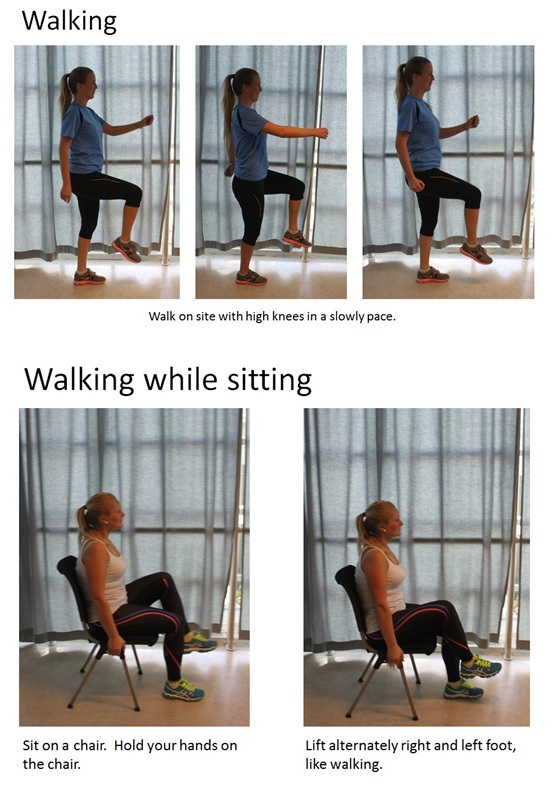
\includegraphics[scale=0.7]{Walking.jpg}
\label{app:walking}
\end{figure} 

\begin{figure} [H]
\centering
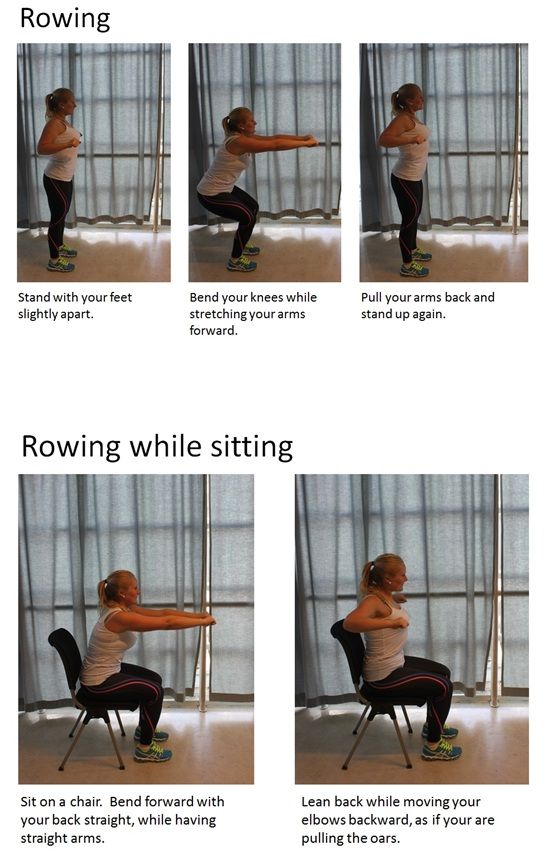
\includegraphics[scale=0.7]{Rowing.jpg}
\label{app:rowing}
\end{figure}

\begin{figure} [H]
\centering
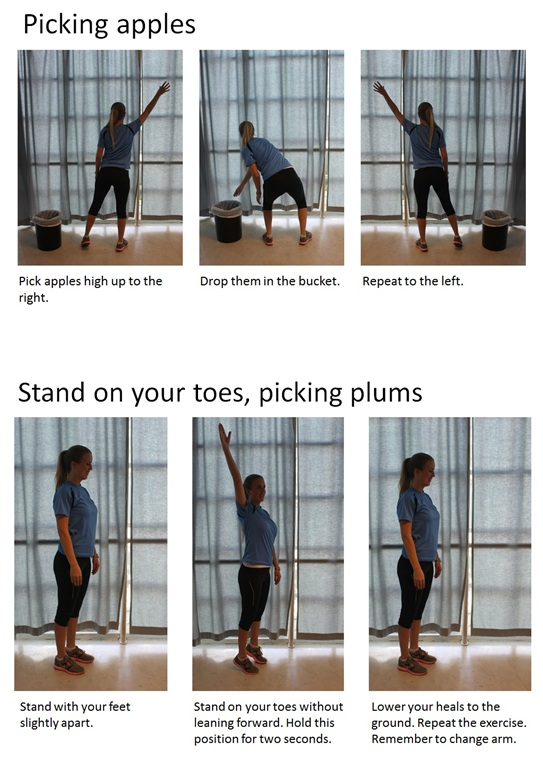
\includegraphics[scale=0.7]{PickingApples.jpg}
\label{app:pickingapplesApp}
\end{figure}

\begin{figure} [H]
\centering
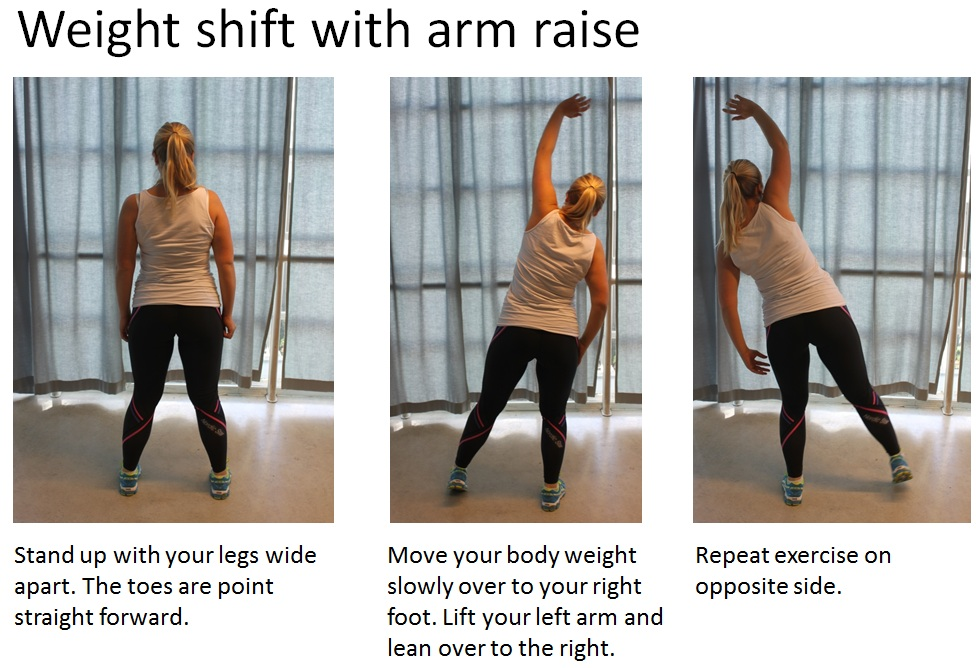
\includegraphics[scale=0.8]{WeightShift.jpg}
\label{app:weightshift}
\end{figure} 

\begin{figure} [H]
\centering
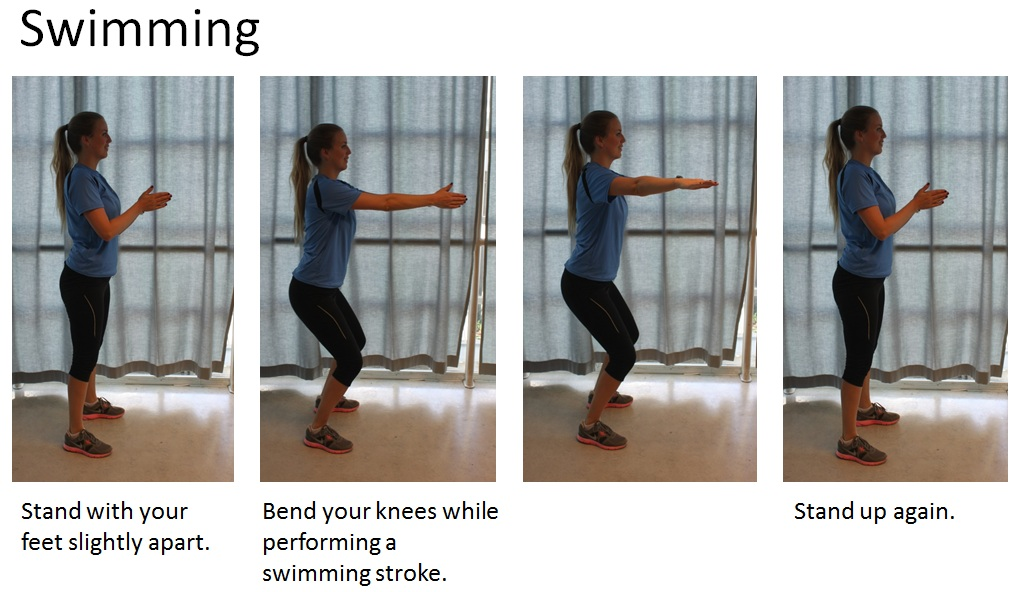
\includegraphics[scale=0.8]{Swimming.jpg}
\label{app:swimming}
\end{figure}

\begin{figure} [H]
\centering
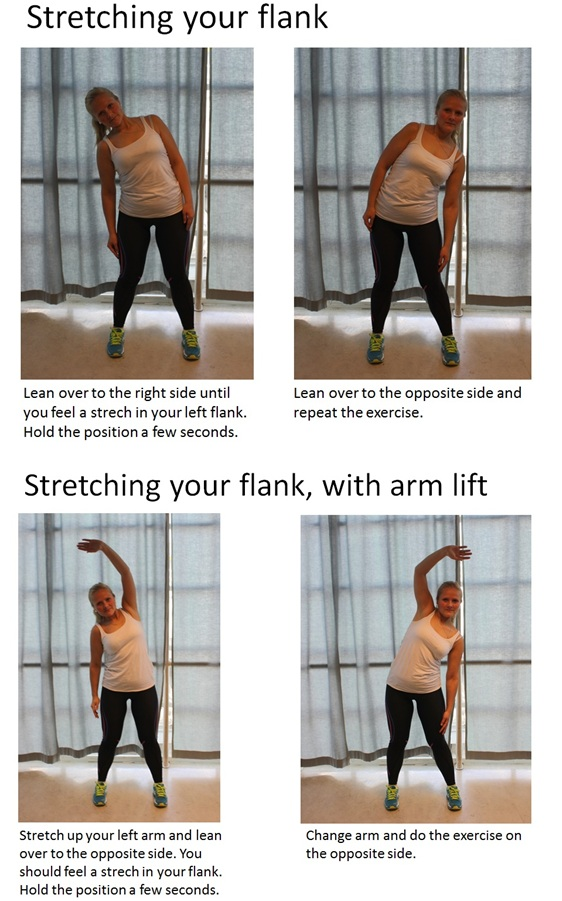
\includegraphics[scale=0.8]{StrechFlank.jpg}
\label{app:stretchflank}
\end{figure} 

\begin{figure} [H]
\centering
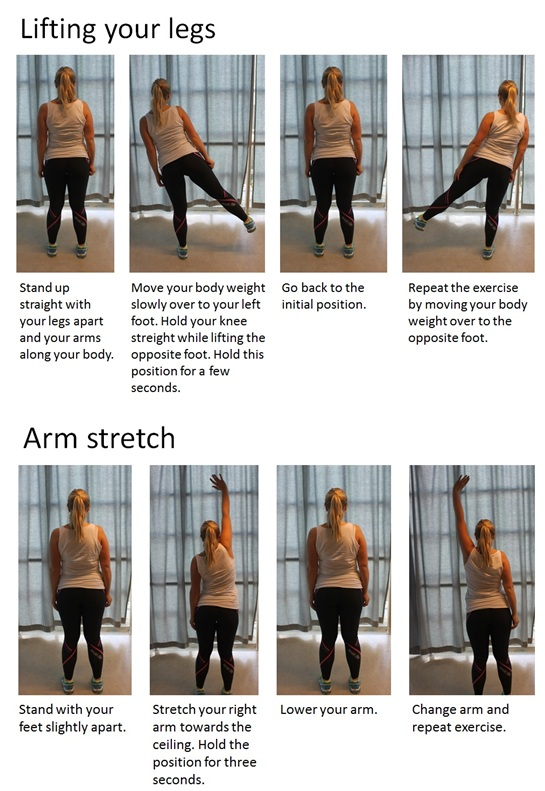
\includegraphics[scale=0.8]{LiftingYourLegs.jpg}
\label{app:liftlegs}
\end{figure} 


\begin{figure} [H]
\centering
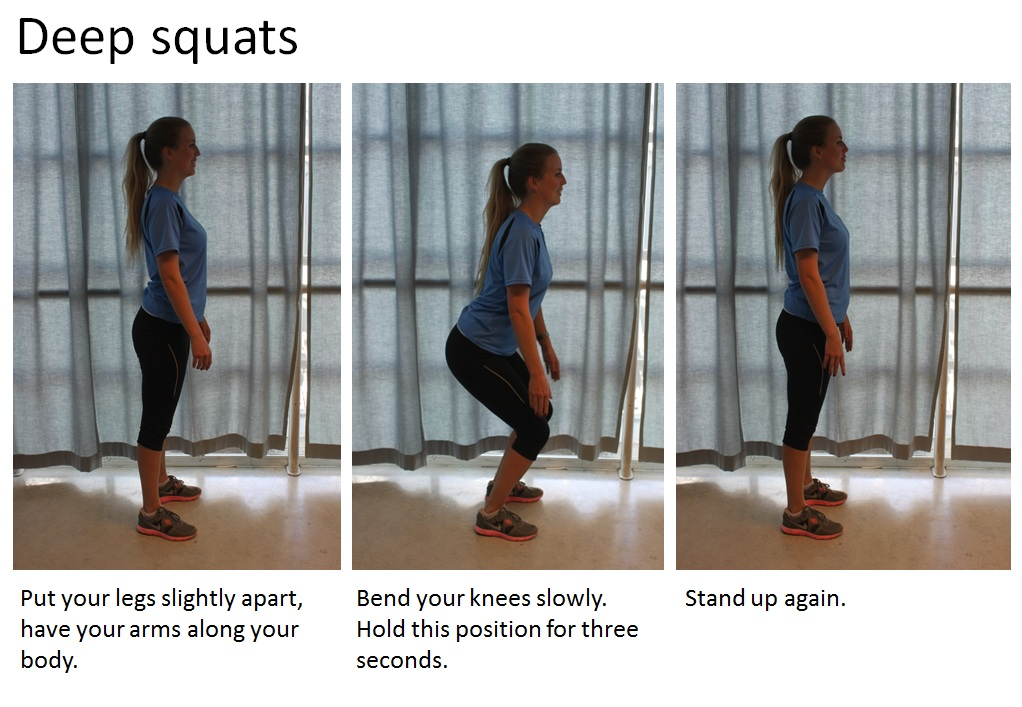
\includegraphics[scale=0.8]{Squats.jpg}
\label{app:squats}
\end{figure}  

\begin{figure} [H]
\centering
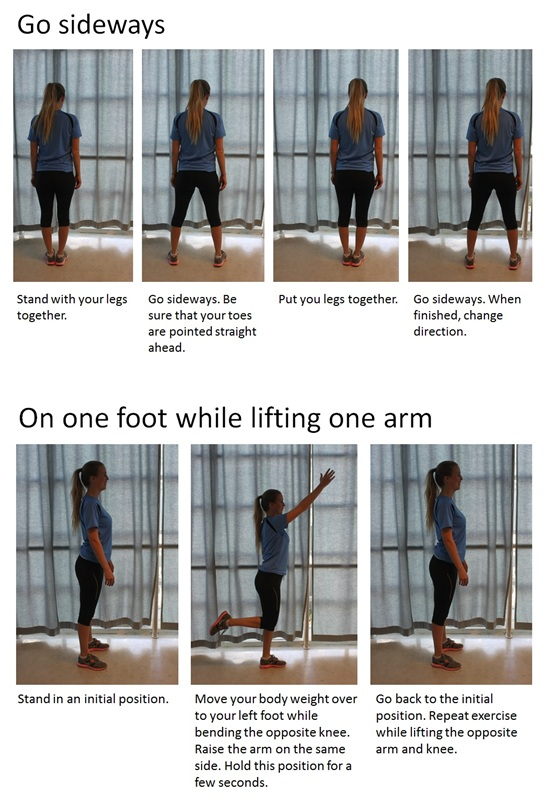
\includegraphics[scale=0.8]{GoSideways.jpg}
\label{app:gosideways}
\end{figure} 

\newpage
\section*{Appendix C - Various Steps from the Original Norwegian Exergame Concept}
\label{app:concept}

\begin{figure} [H]
\centering
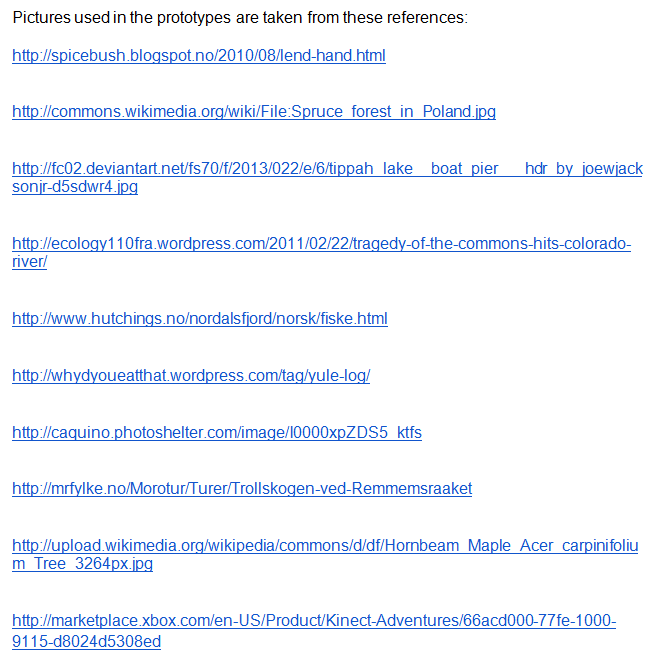
\includegraphics[scale=0.8]{kilderprototype}
\label{fig:kilder}
\end{figure}

\begin{figure} [H]
\centering
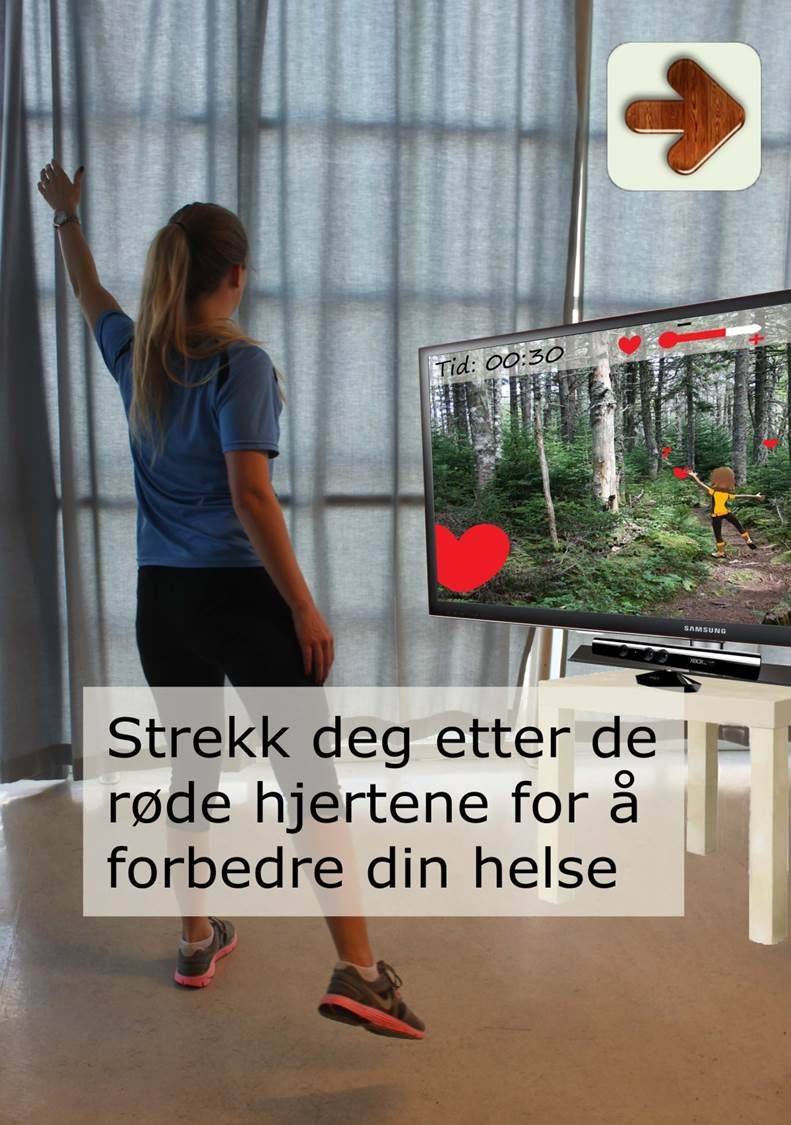
\includegraphics[scale=0.7]{KineIntro.jpg}
\label{fig:kineintroNorsk}
\end{figure}

\begin{figure} [H]
\centering
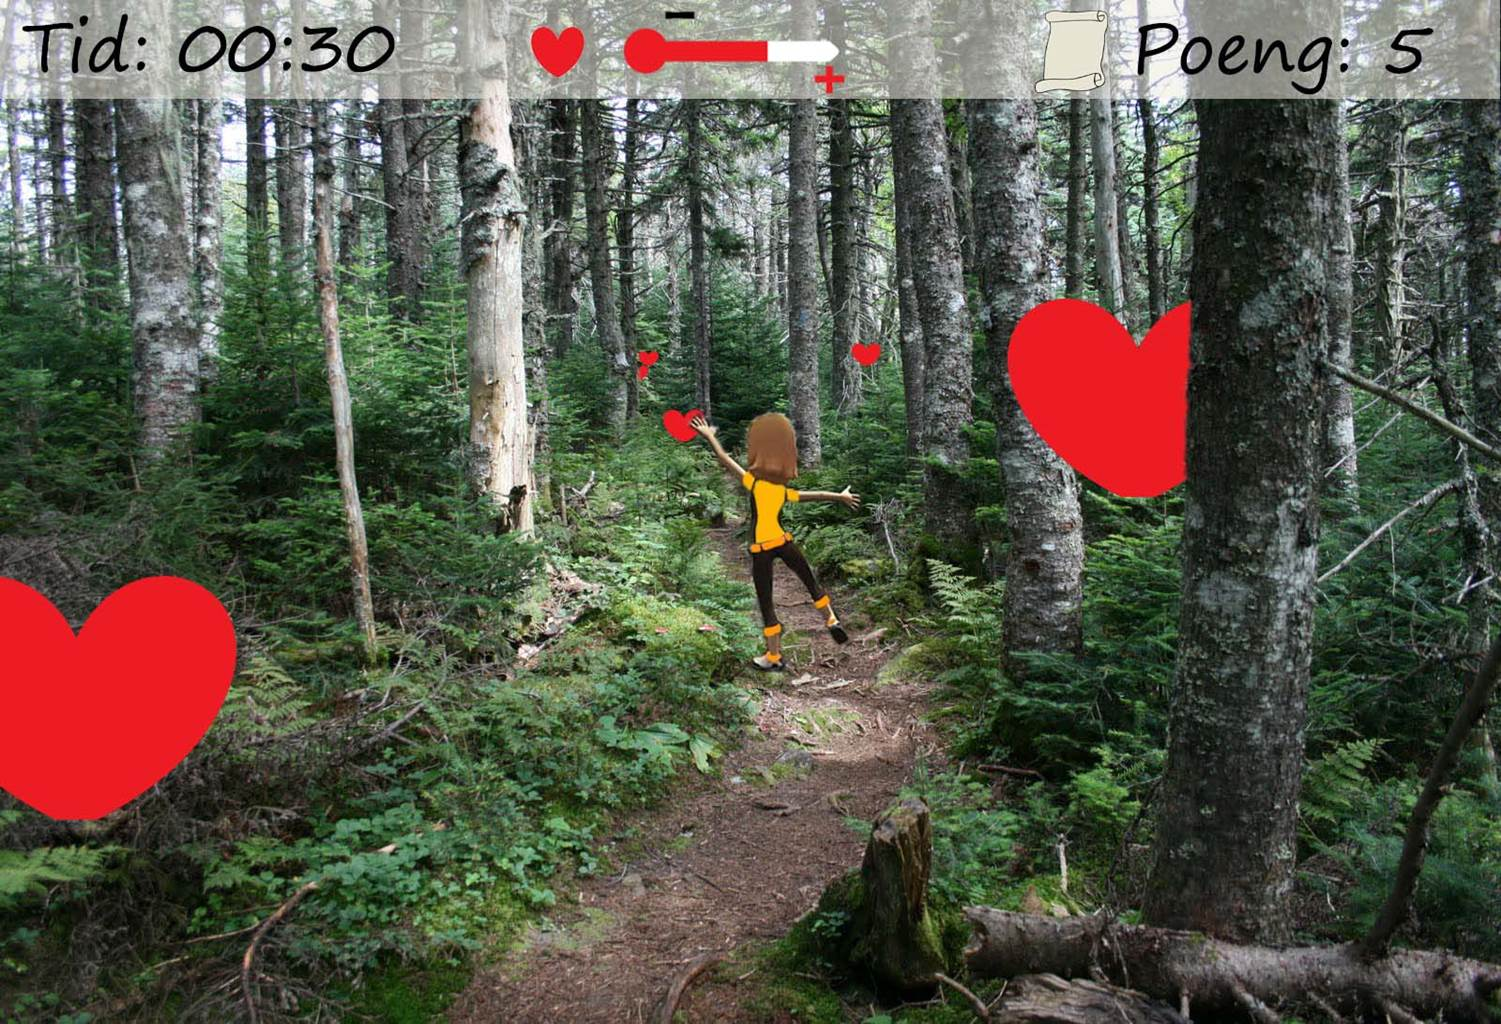
\includegraphics[scale=0.5]{hjerter.jpg}
\label{fig:heartsNorsk}
\end{figure}

\begin{figure} [H]
\centering
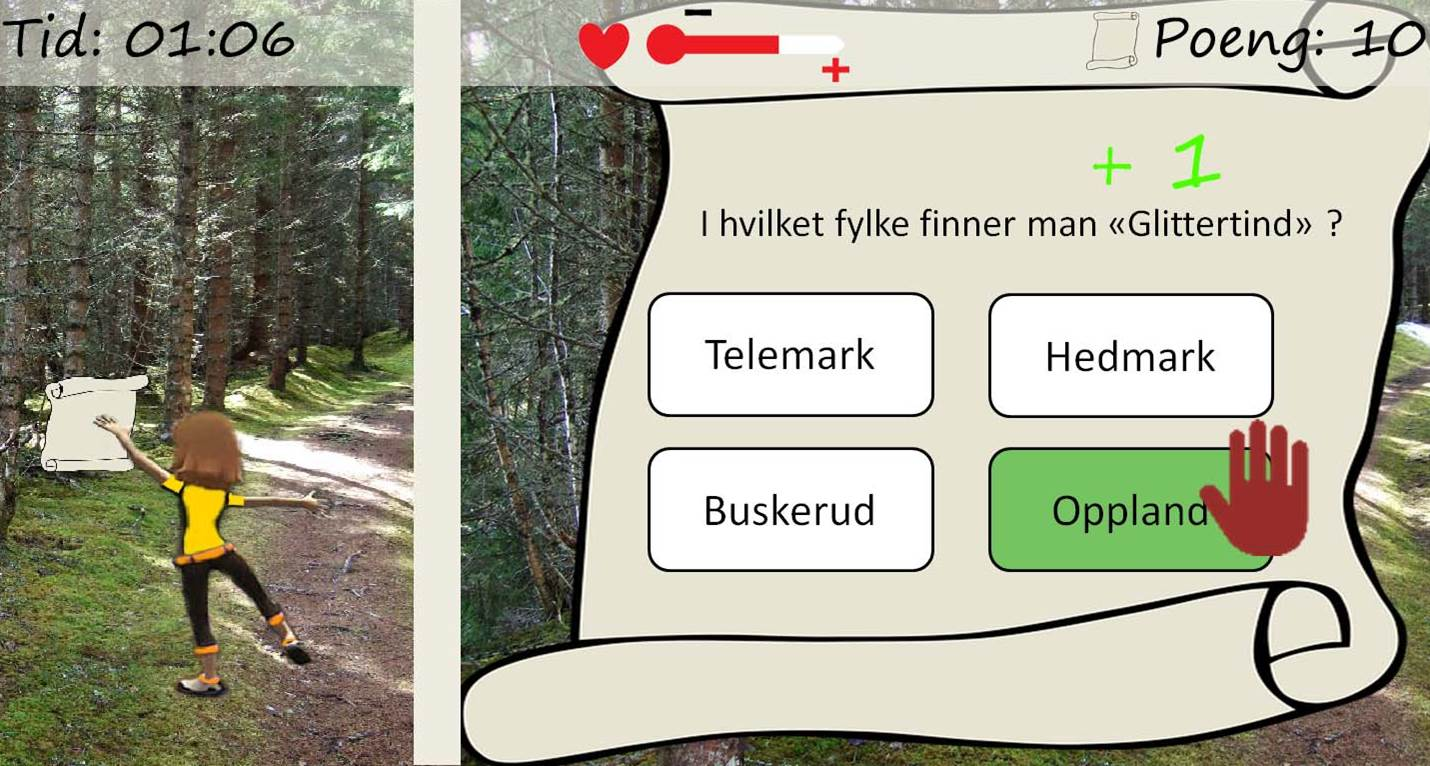
\includegraphics[scale=0.25]{quiz.jpg}
\label{fig:quizapp}
\end{figure} 

\begin{figure} [H]
\centering
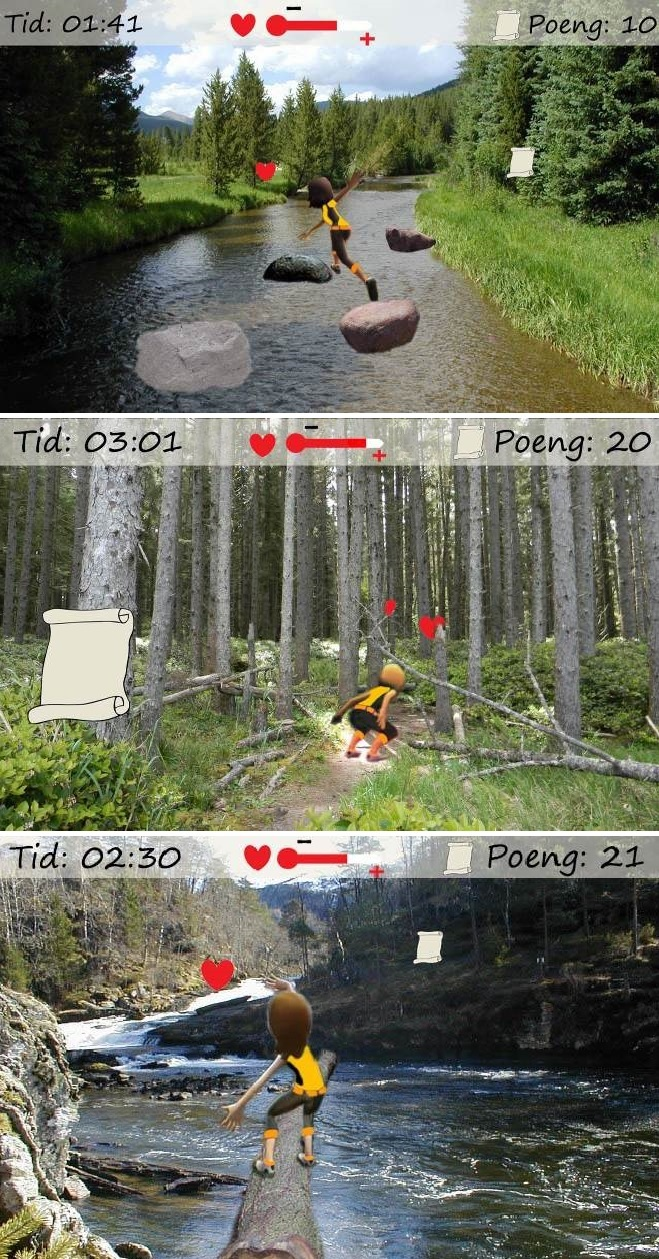
\includegraphics[scale=0.45]{hindring1.jpg}
\label{fig:hindring1Norsk}
\end{figure}

\begin{figure} [H]
\centering
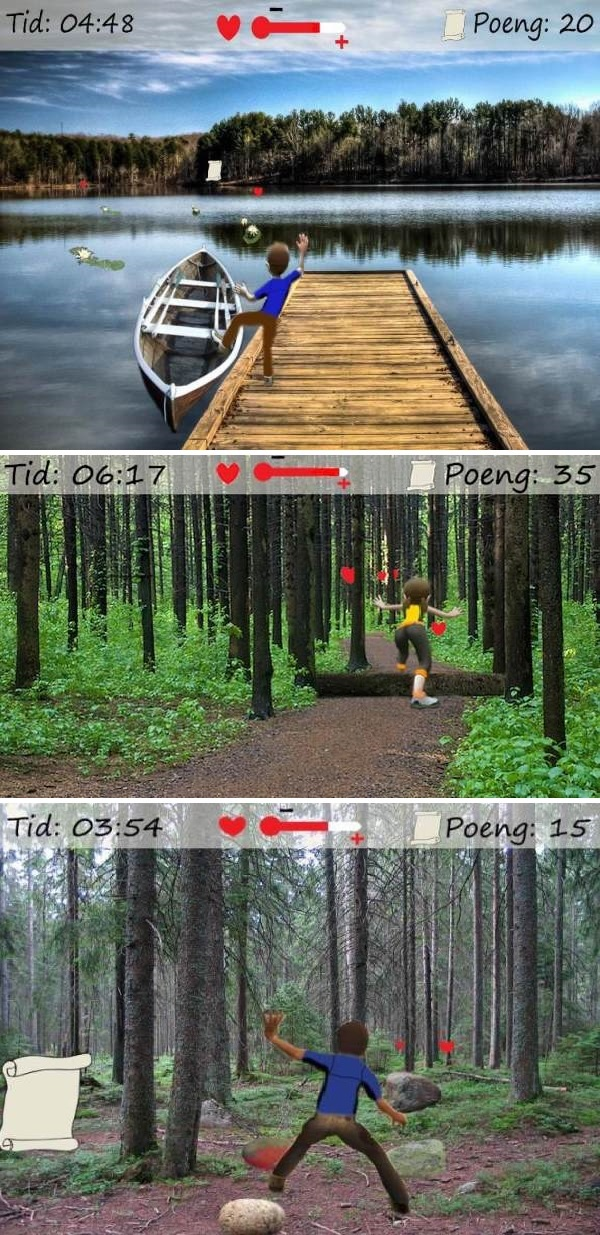
\includegraphics[scale=0.45]{hindring2.jpg}
\label{fig:hindring2Norsk}
\end{figure}

\begin{figure} [H]
\centering
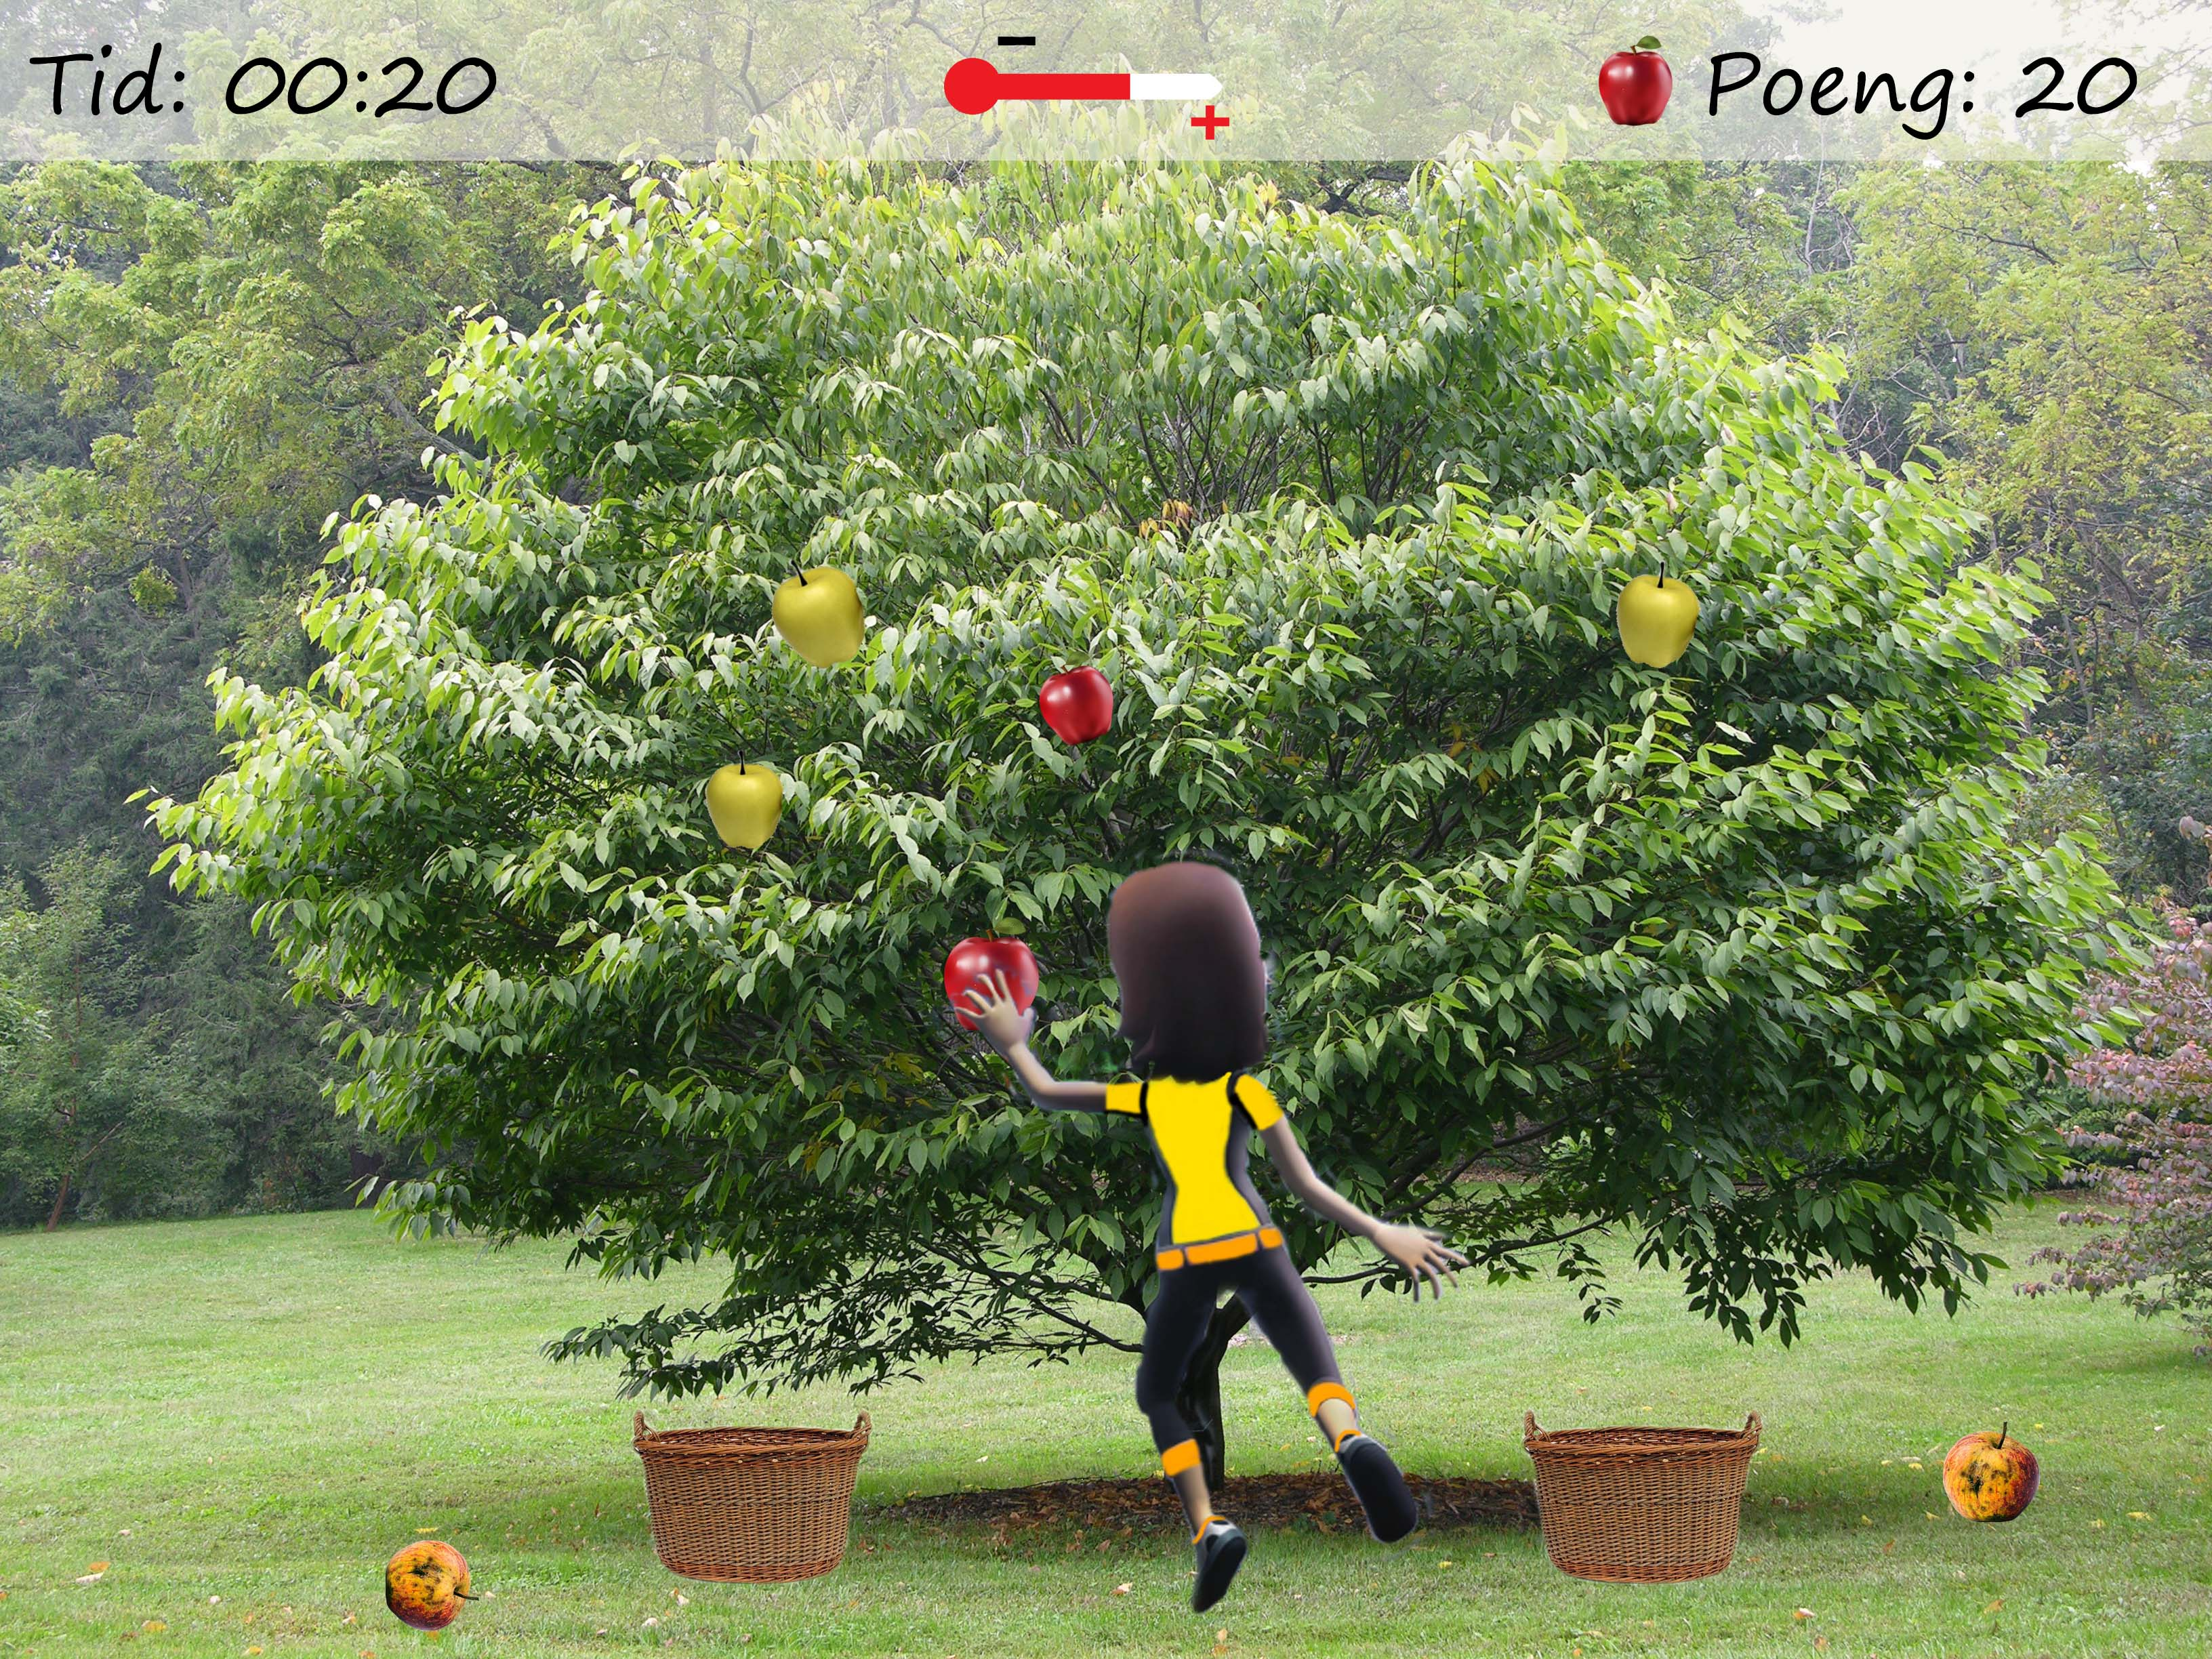
\includegraphics[scale=0.1]{gameappletree.jpg}
\label{fig:appleStretchNorsk}
\end{figure}

\begin{figure} [H]
\centering
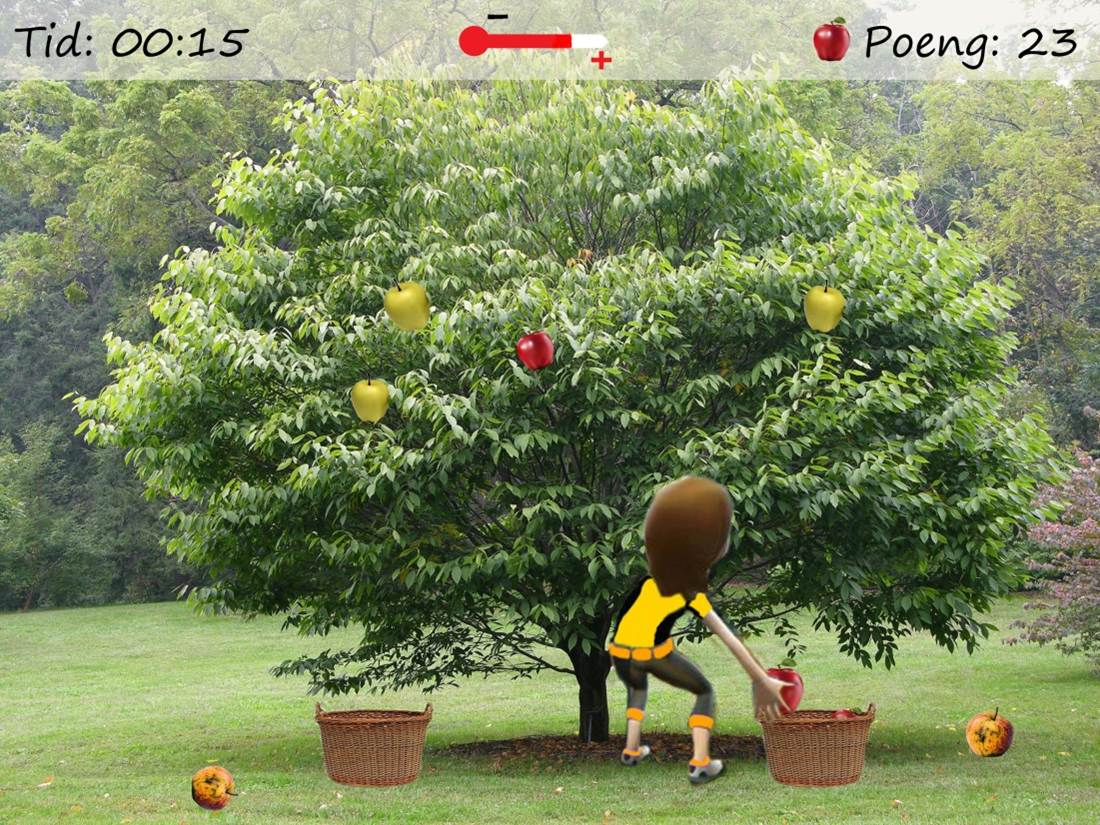
\includegraphics[scale=0.45]{squateple.jpg}
\label{fig:appleSquatNorsk}
\end{figure}

\begin{figure} [H]
\centering
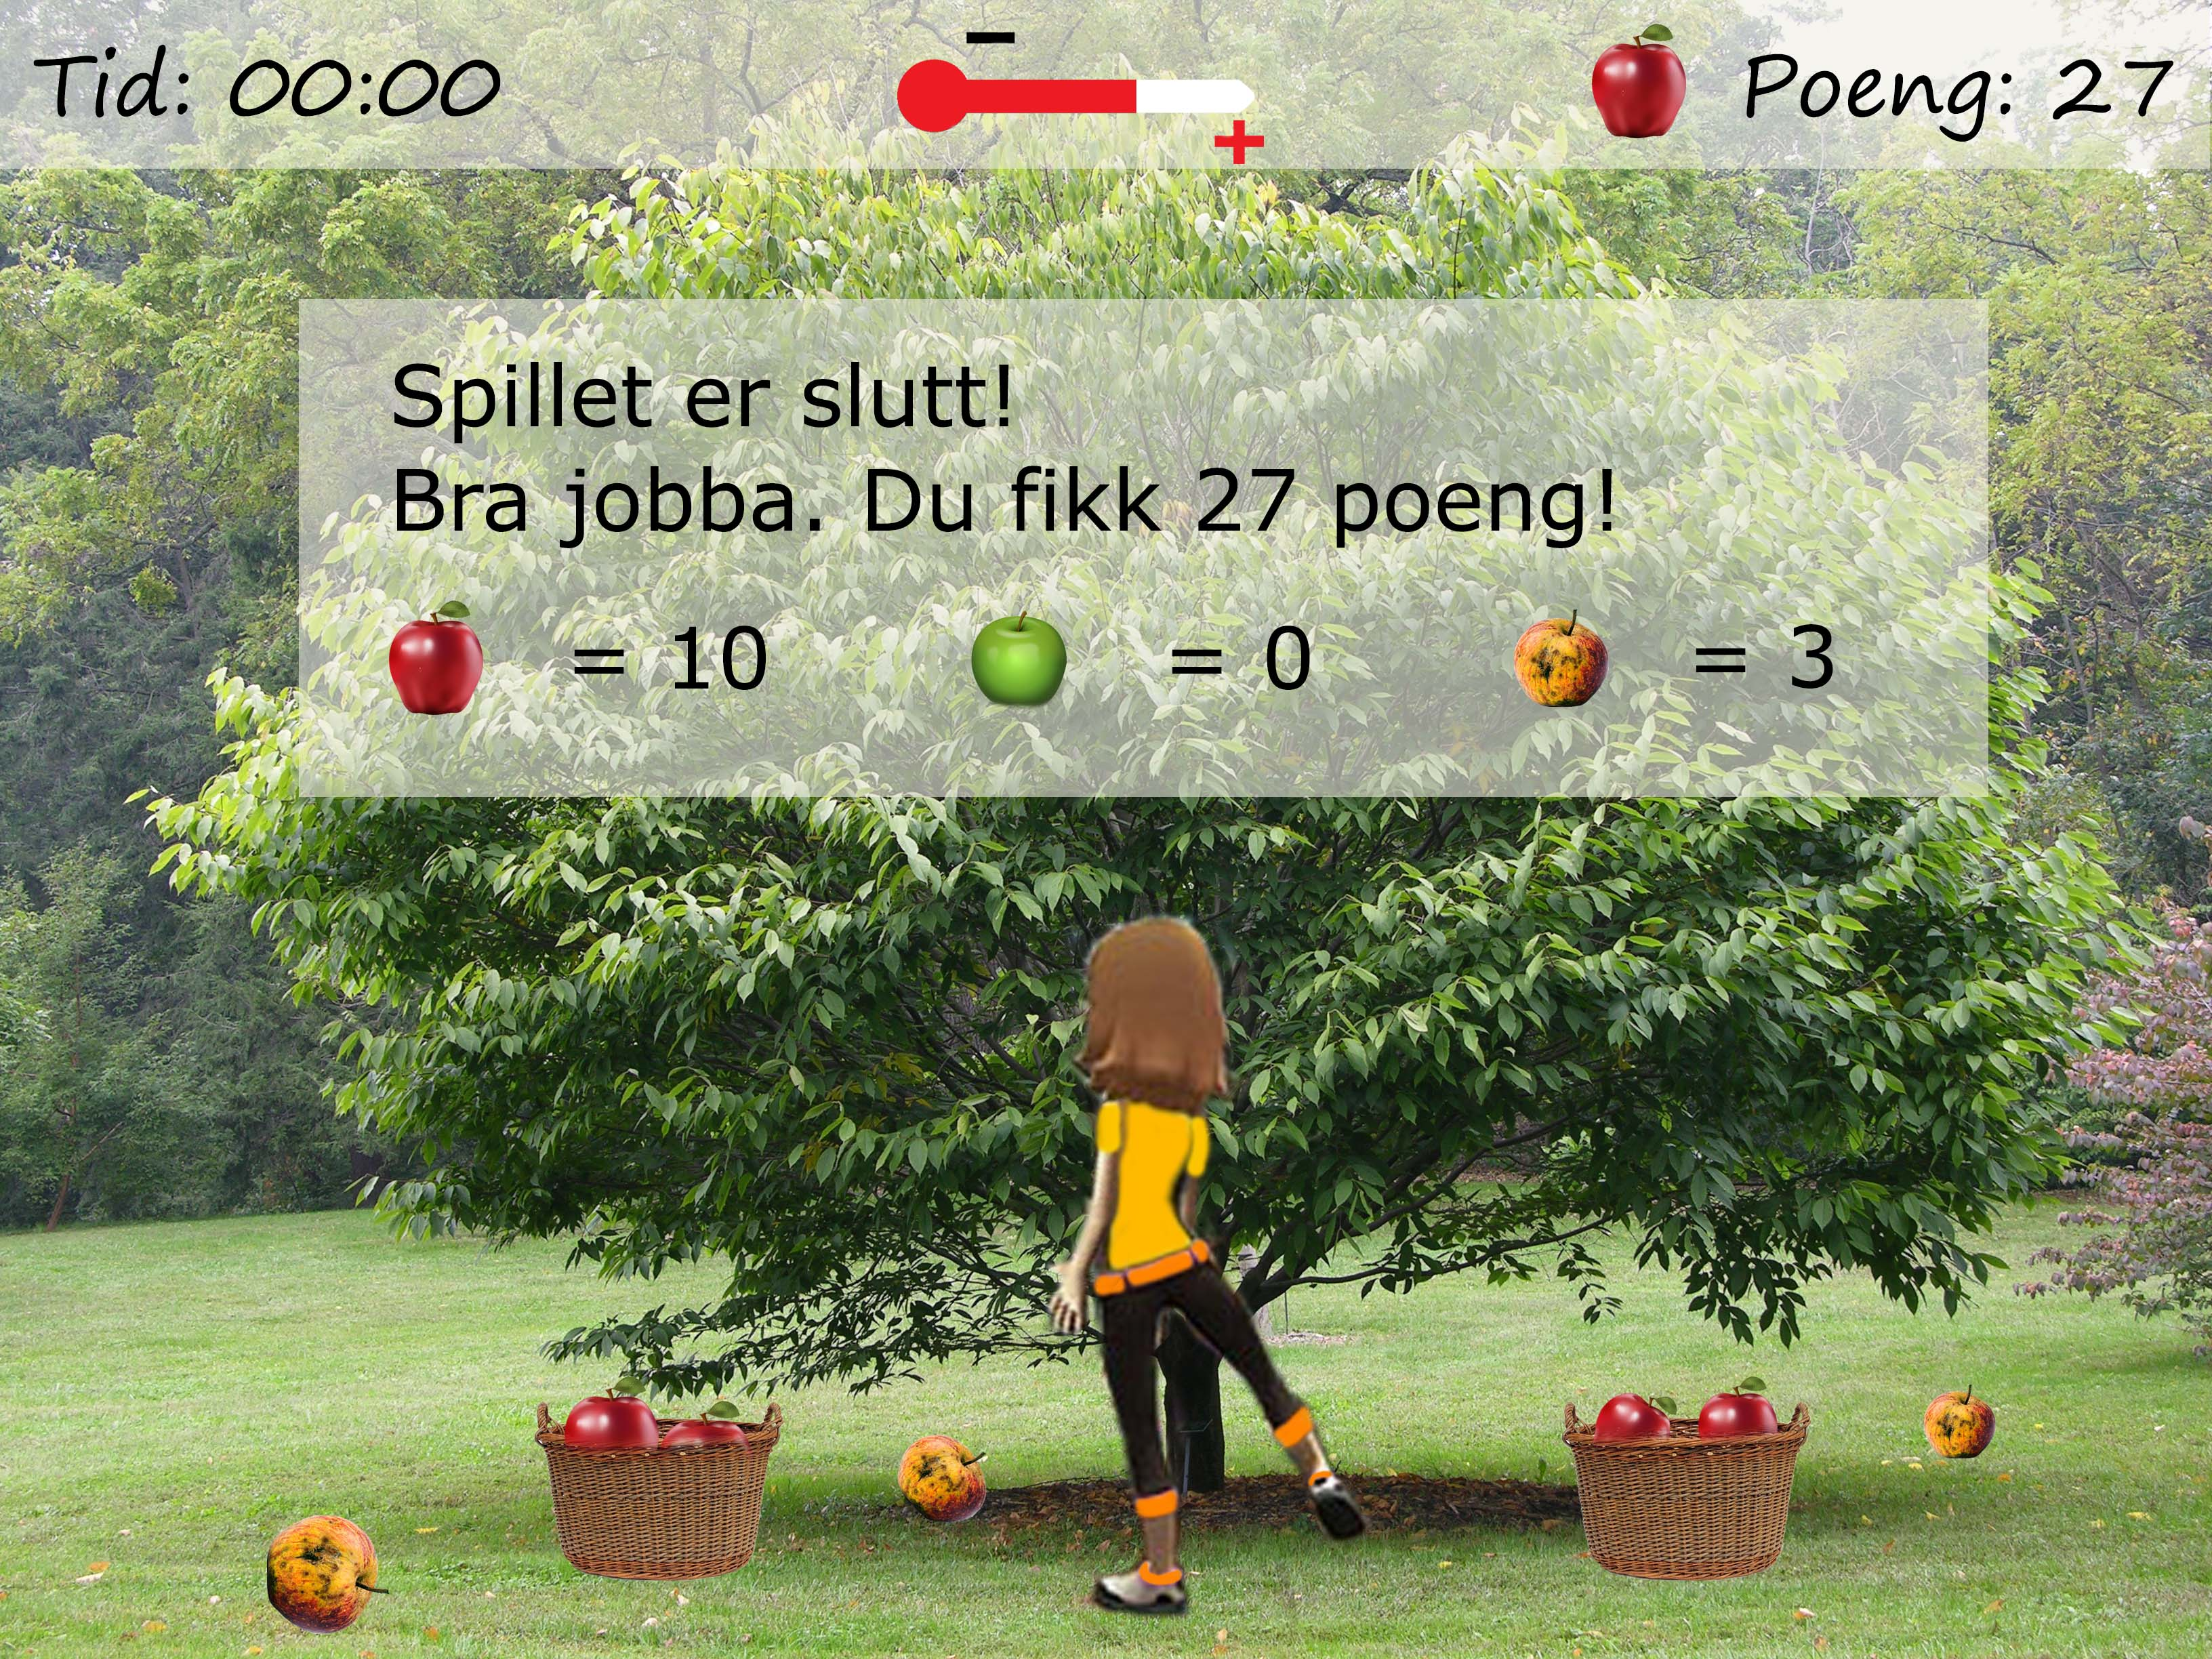
\includegraphics[scale=0.1]{appletreeend.jpg}
\label{fig:appleOverNorsk}
\end{figure}

\begin{figure} [H]
\centering
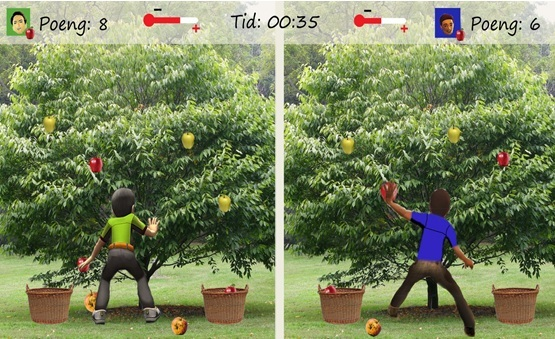
\includegraphics[scale=0.8]{multiplayereple.jpg}
\label{fig:appleMultiplayerNorsk}
\end{figure}

\begin{figure} [H]
\centering
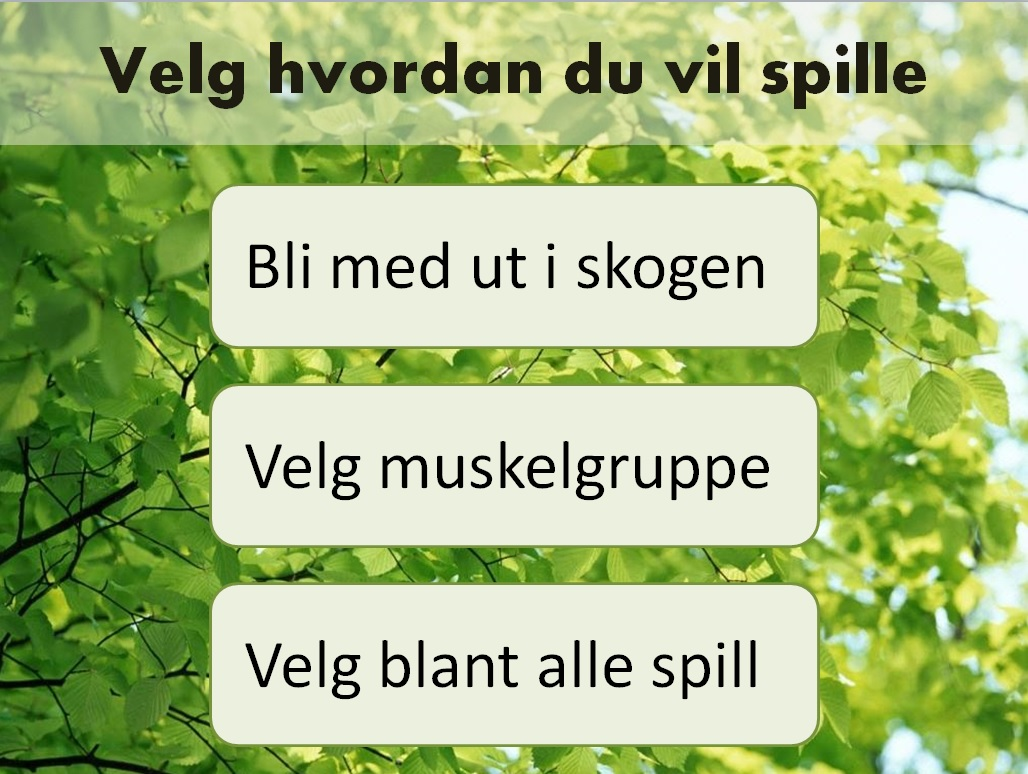
\includegraphics[scale=0.45]{menuStart.jpg}
\label{fig:menuStartNorsk}
\end{figure} 

\begin{figure} [H]
\centering
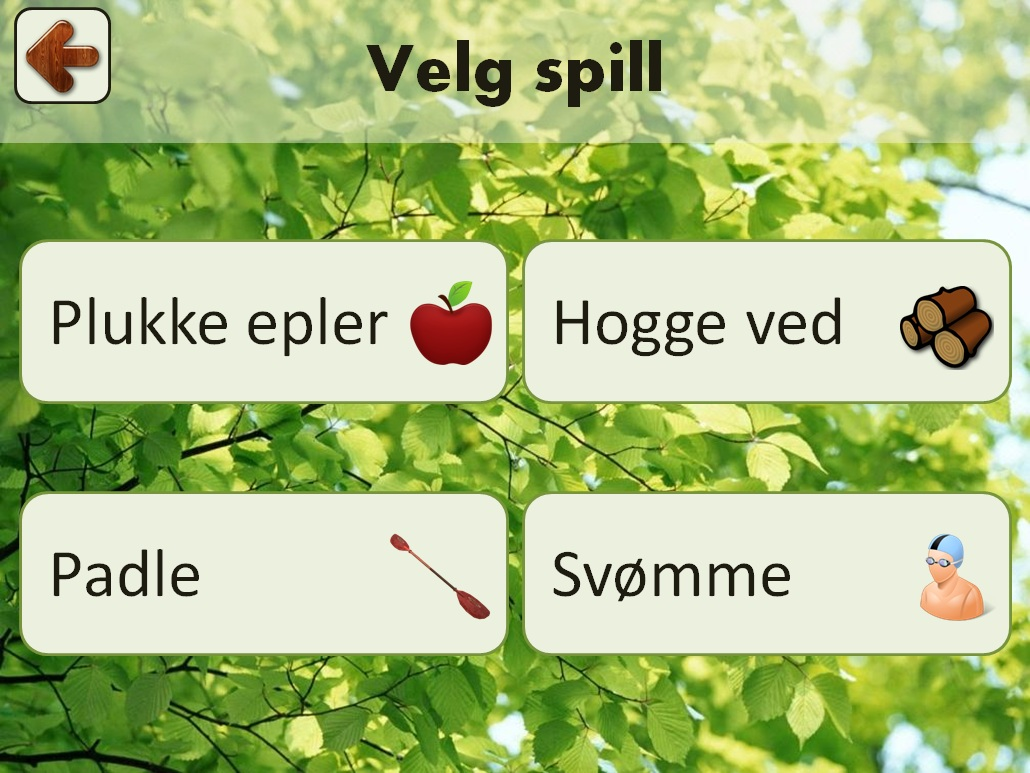
\includegraphics[scale=0.4]{VelgSpill.jpg}
\label{velgSpillNorsk}
\end{figure}

\begin{figure} [H]
\centering
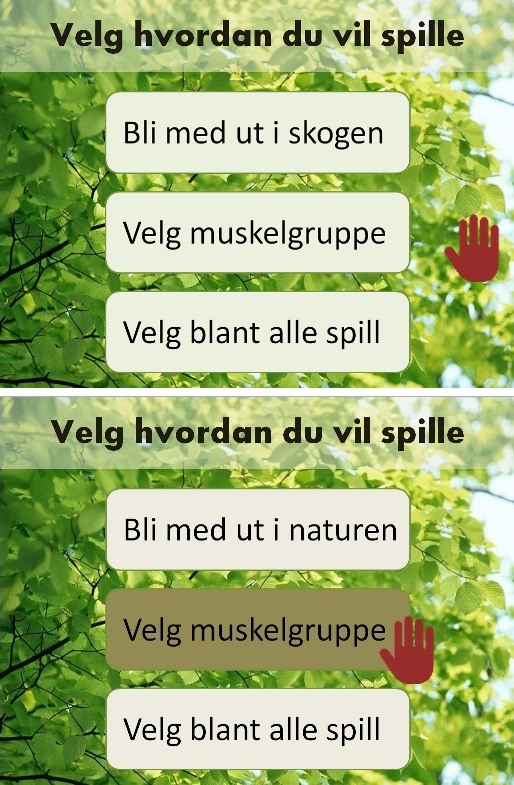
\includegraphics[scale=0.5]{menuAvatarAction.jpg}
\label{fig:avatarActionNorsk}
\end{figure} 

\begin{figure} [H]
\centering
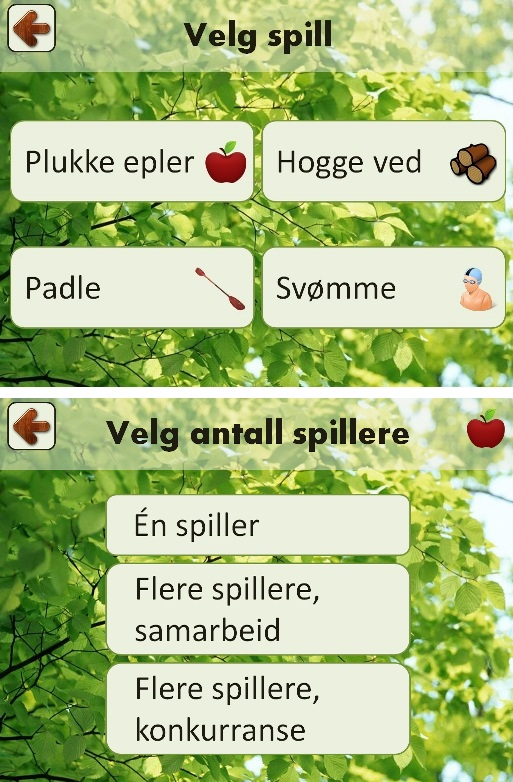
\includegraphics[scale=0.5]{IconEple.jpg}
\label{fig:iconEpleNorsk}
\end{figure} 

\begin{figure} [H]
\centering
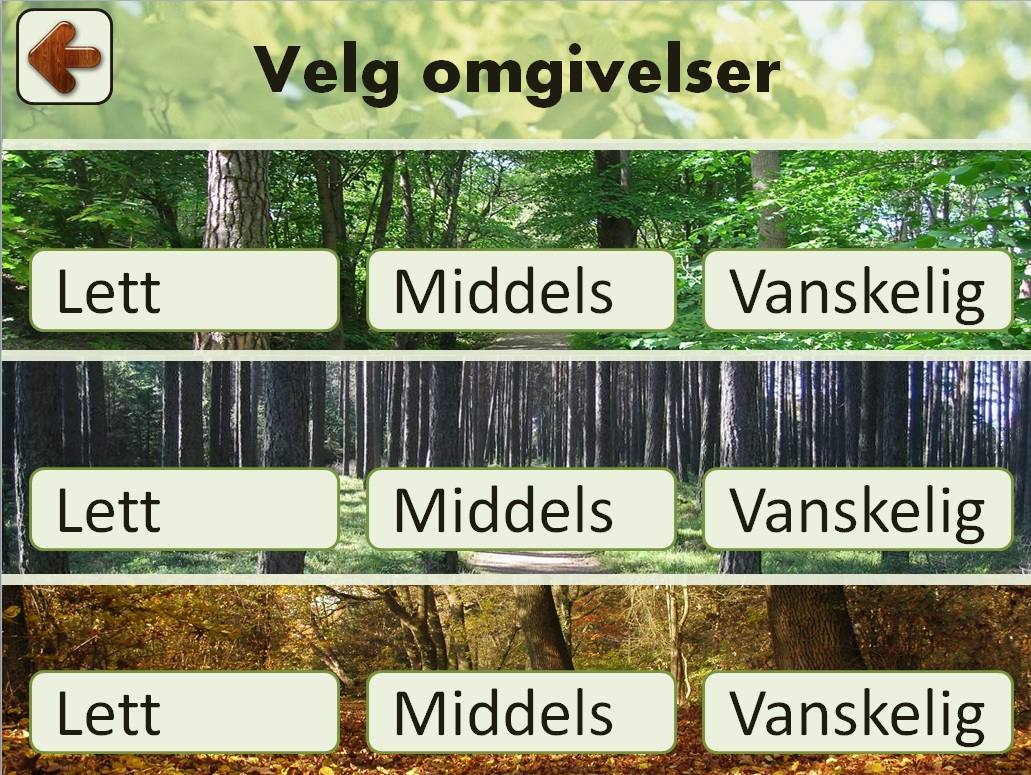
\includegraphics[scale=0.45]{VelgOmgivelser.jpg}
\label{fig:omgivelseNivaaNorsk}
\end{figure}

\begin{figure} [H]
\centering
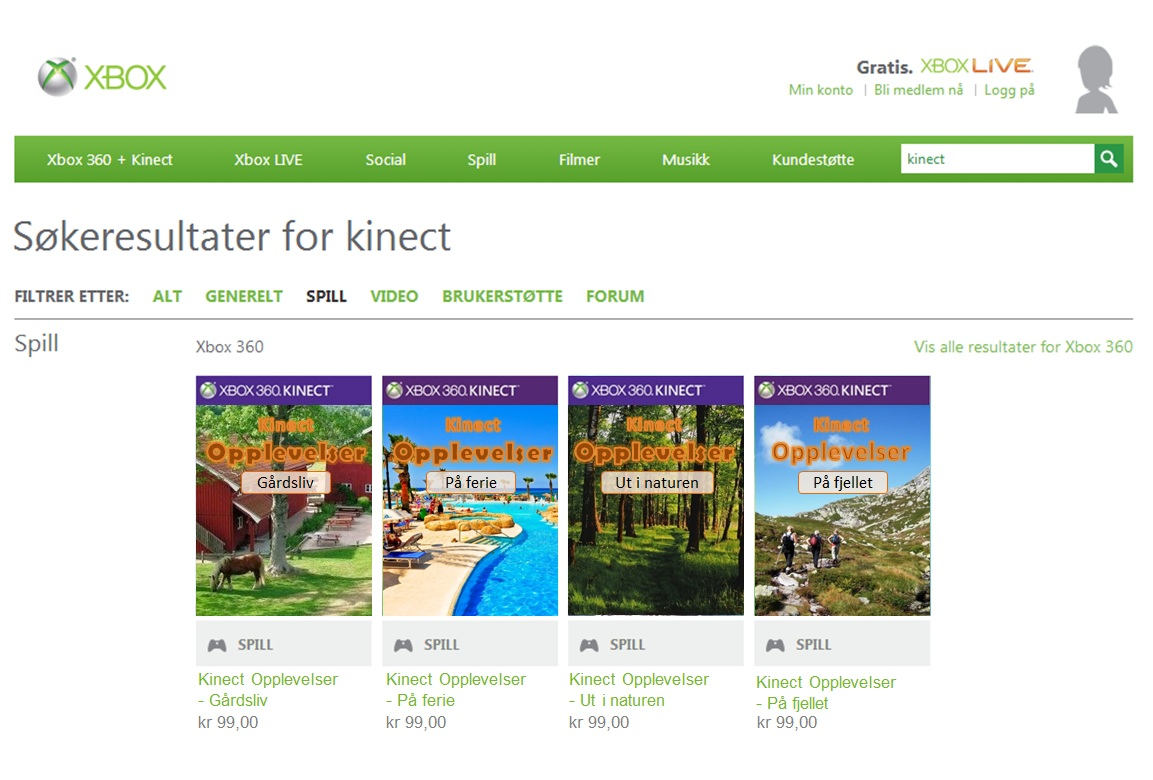
\includegraphics[scale=0.5, angle=90]{SpillXboxNYNY.jpg}
\label{fig:videogameseriesHeleNorsk}
\end{figure}

\newpage
\section*{Appendix D - Review of the Original Norwegian Menu}
\label{app:menureview}

The figures shown in Appendix C shows a review of the original prototypes of the menu. This menu was presented for the informants in workshop 2, and is therefore in Norwegian. The menu review starts with the choice on how to play. The player chooses to play according to a preferred muscle group. A selection of single games are shown, where the player chooses "picking apples". The menu shows a start, middle, and end scene from this game. When finished, the player chooses to change number of players from single player to multi player.  

\begin{figure} [H]
\centering
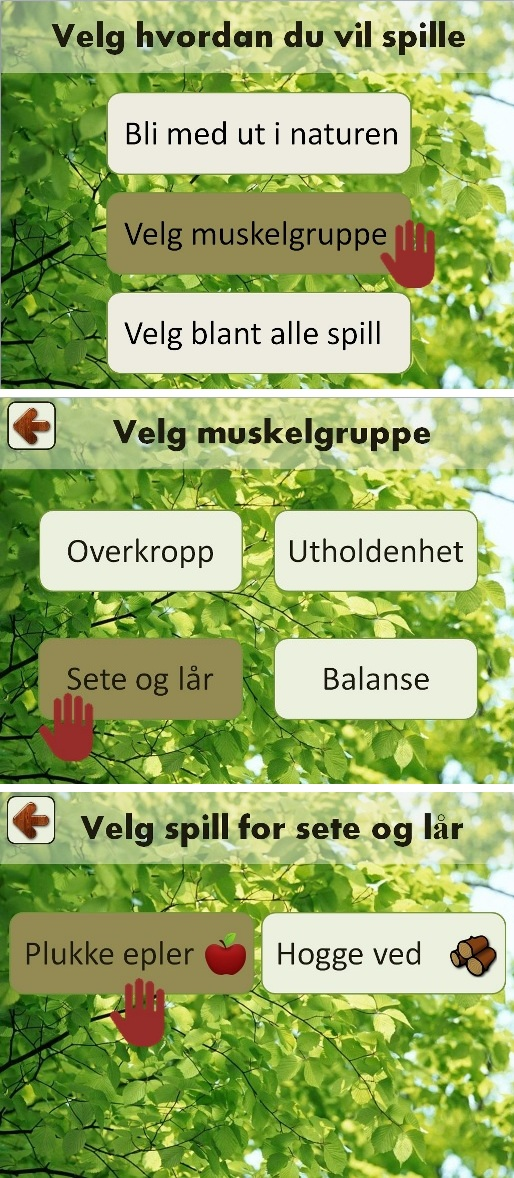
\includegraphics[scale=0.45]{menuStep1.jpg}
\label{app:menu1Norsk}
\end{figure}

\begin{figure} [H]
\centering
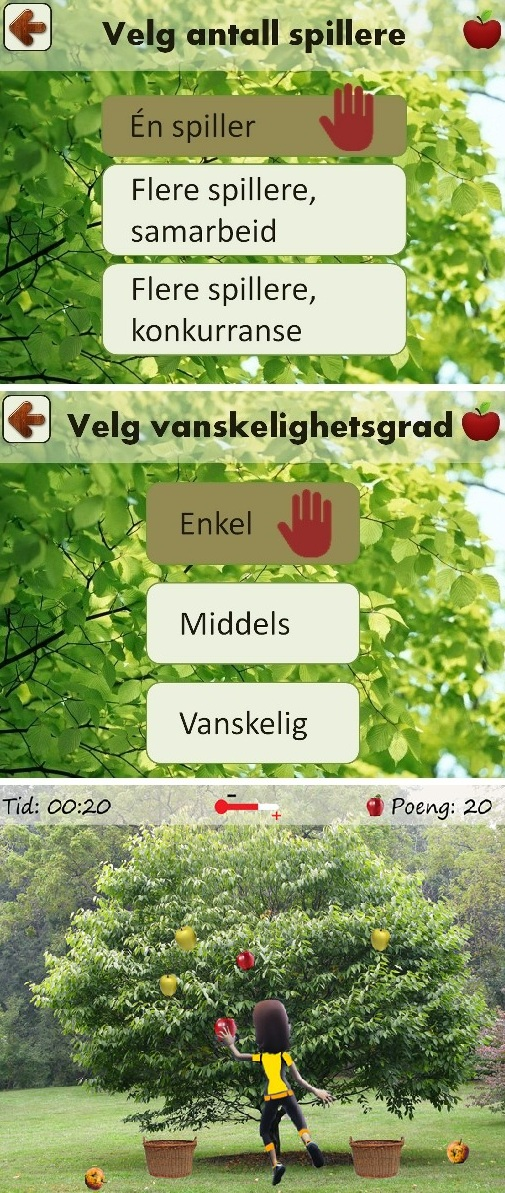
\includegraphics[scale=0.45]{menuStep2.jpg}
\label{app:menu2Norsk}
\end{figure}

\begin{figure} [H]
\centering
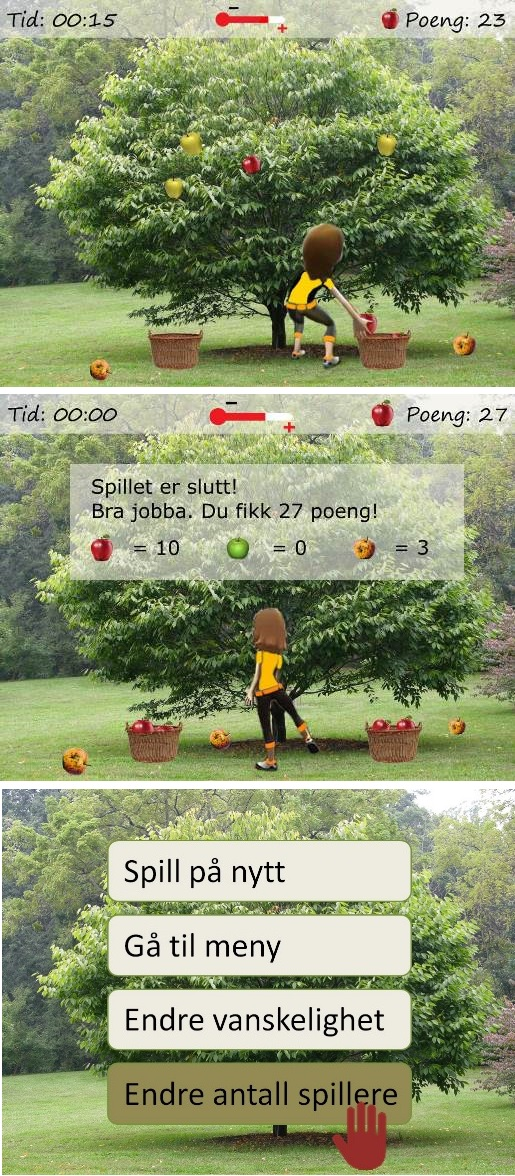
\includegraphics[scale=0.45]{menuStep3.jpg}
\label{app:menu3Norsk}
\end{figure}

\begin{figure} [H]
\centering
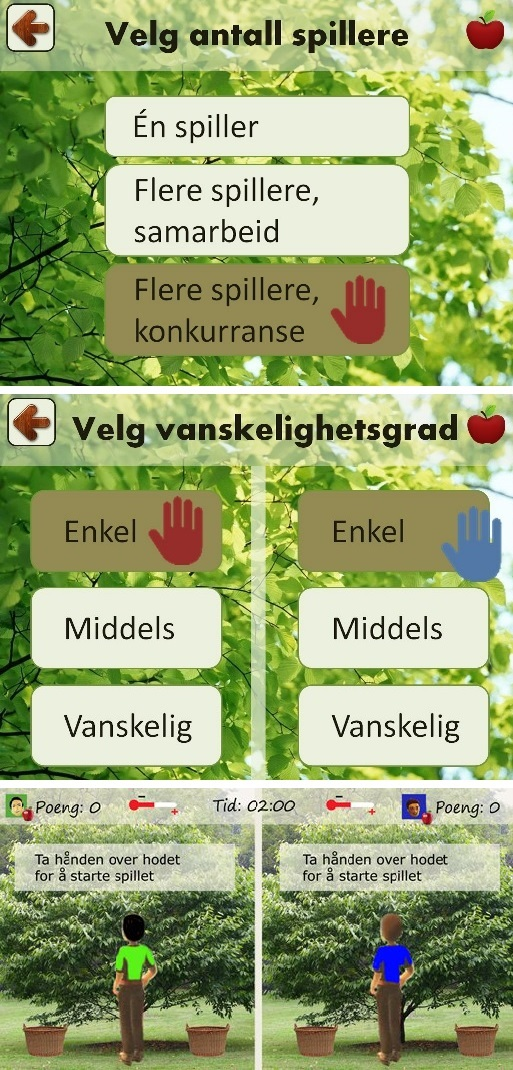
\includegraphics[scale=0.45]{menuStep4.jpg}
\label{app:menu4Norsk}
\end{figure}

\newpage
\section*{Appendix E - Response on our Application to NSD}
\label{app:presentation}
\begin{figure}[H] 
\centering{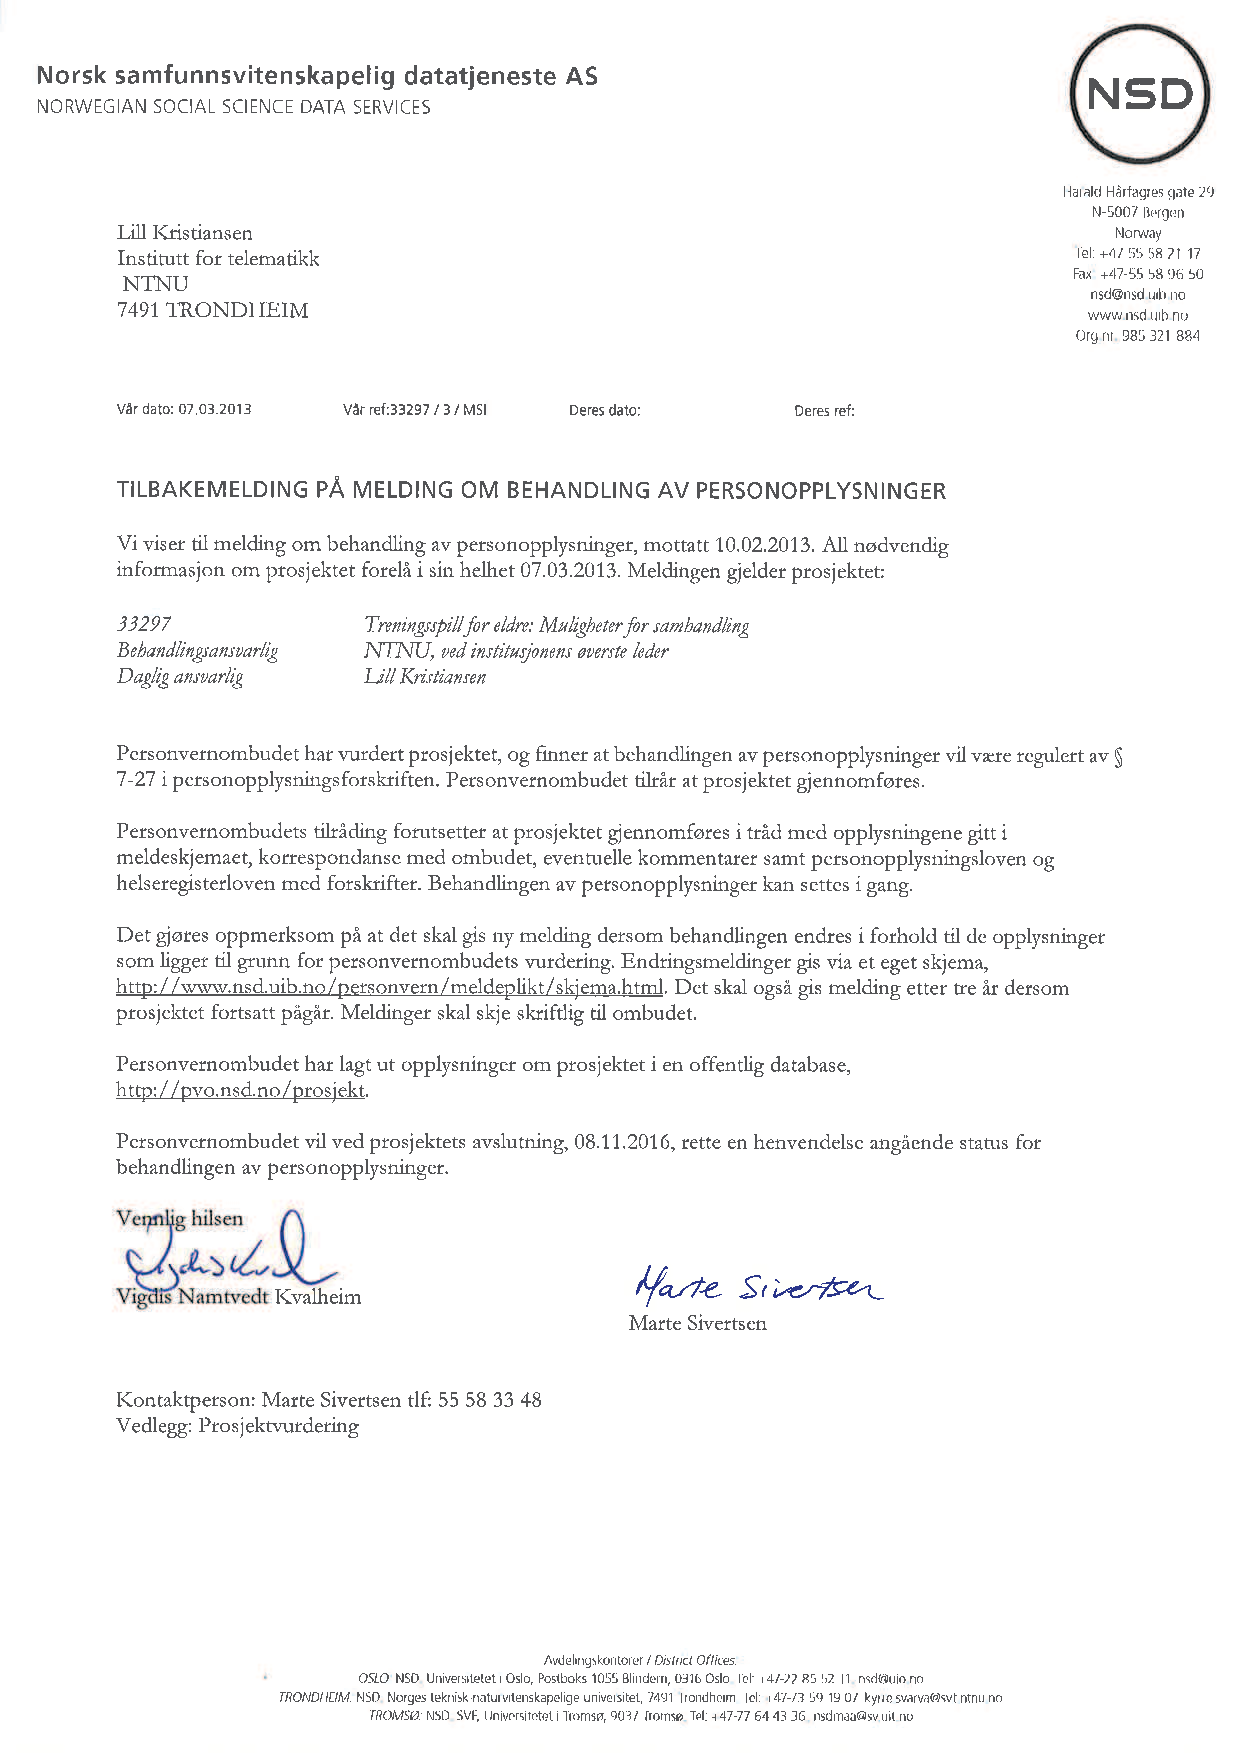
\includegraphics[scale=0.6]{NSD1.pdf}}
\end{figure}  
\begin{figure}[H] 
\centering{
\includegraphics[scale=0.6]{NSD2.pdf}}
\end{figure} 

\newpage
\section*{Appendix F - Informed Consent}
\label{app:infoConsent}
\begin{figure}[H] 
\centering{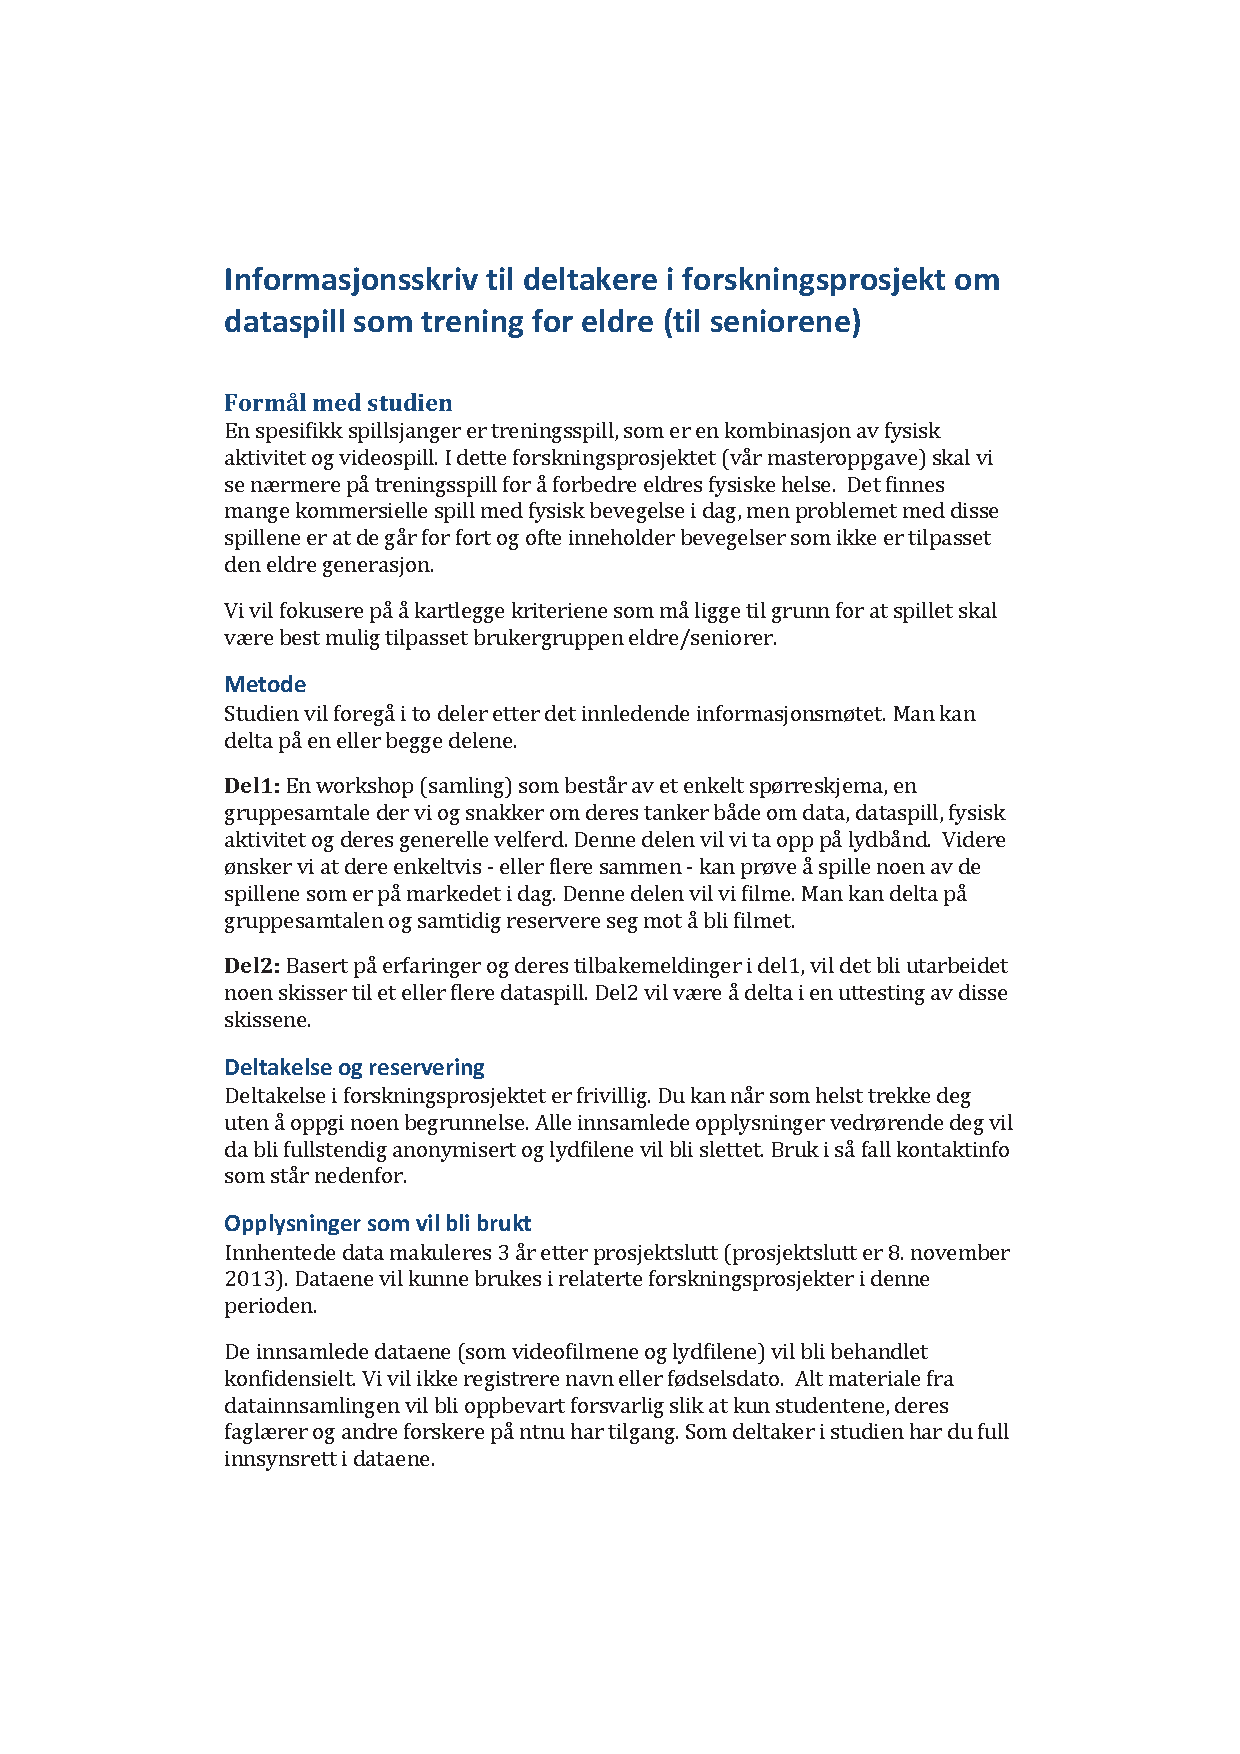
\includegraphics[scale=0.65]{Info-samtykke-til-senior1.pdf}}
\end{figure}  
\begin{figure}[H] 
\centering{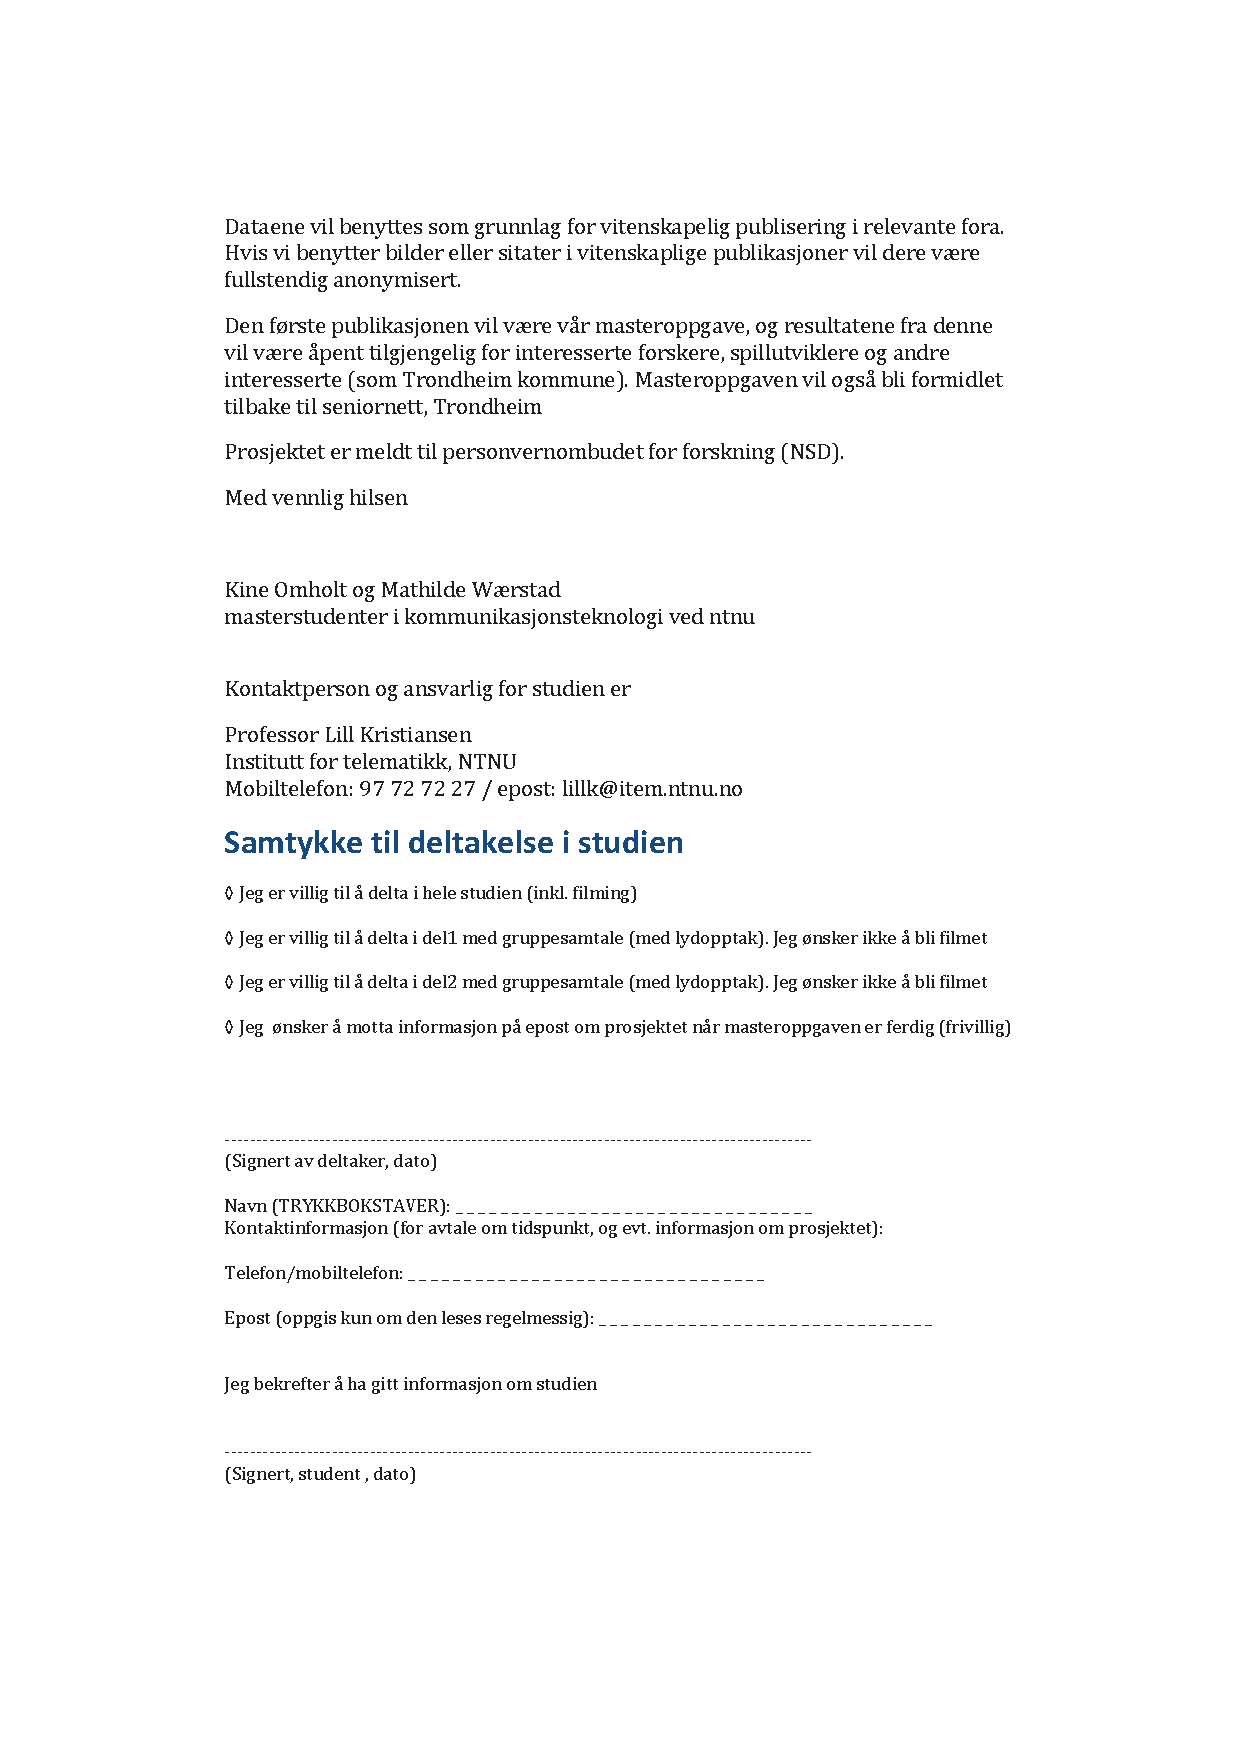
\includegraphics[scale=0.65]{Info-samtykke-til-senior2.pdf}}
\end{figure} 

\newpage
\section*{Appendix G - Questionnaire}
\label{app:questionnaire}
\begin{figure}[H] 
\centering{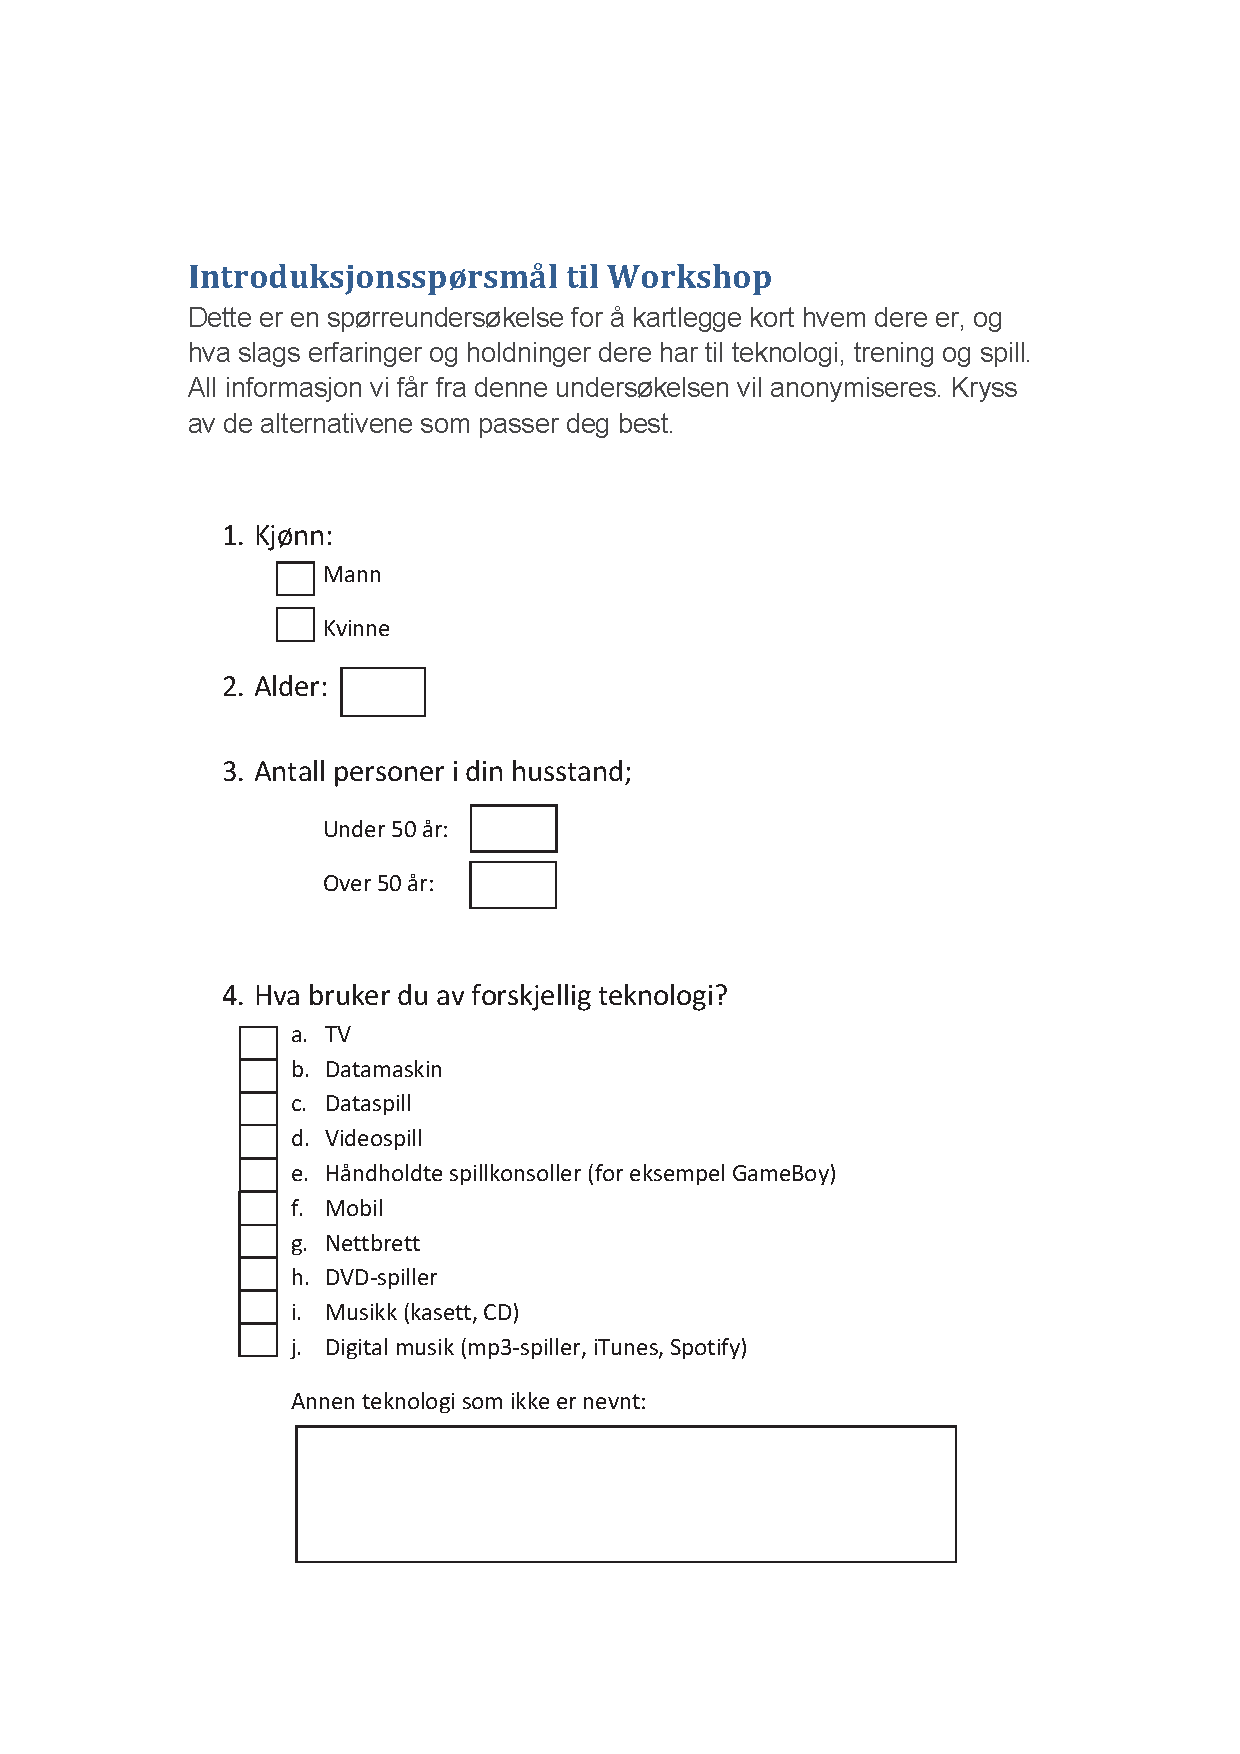
\includegraphics[scale=0.65]{SU1.pdf}}
\end{figure}  
\begin{figure}[H] 
\centering{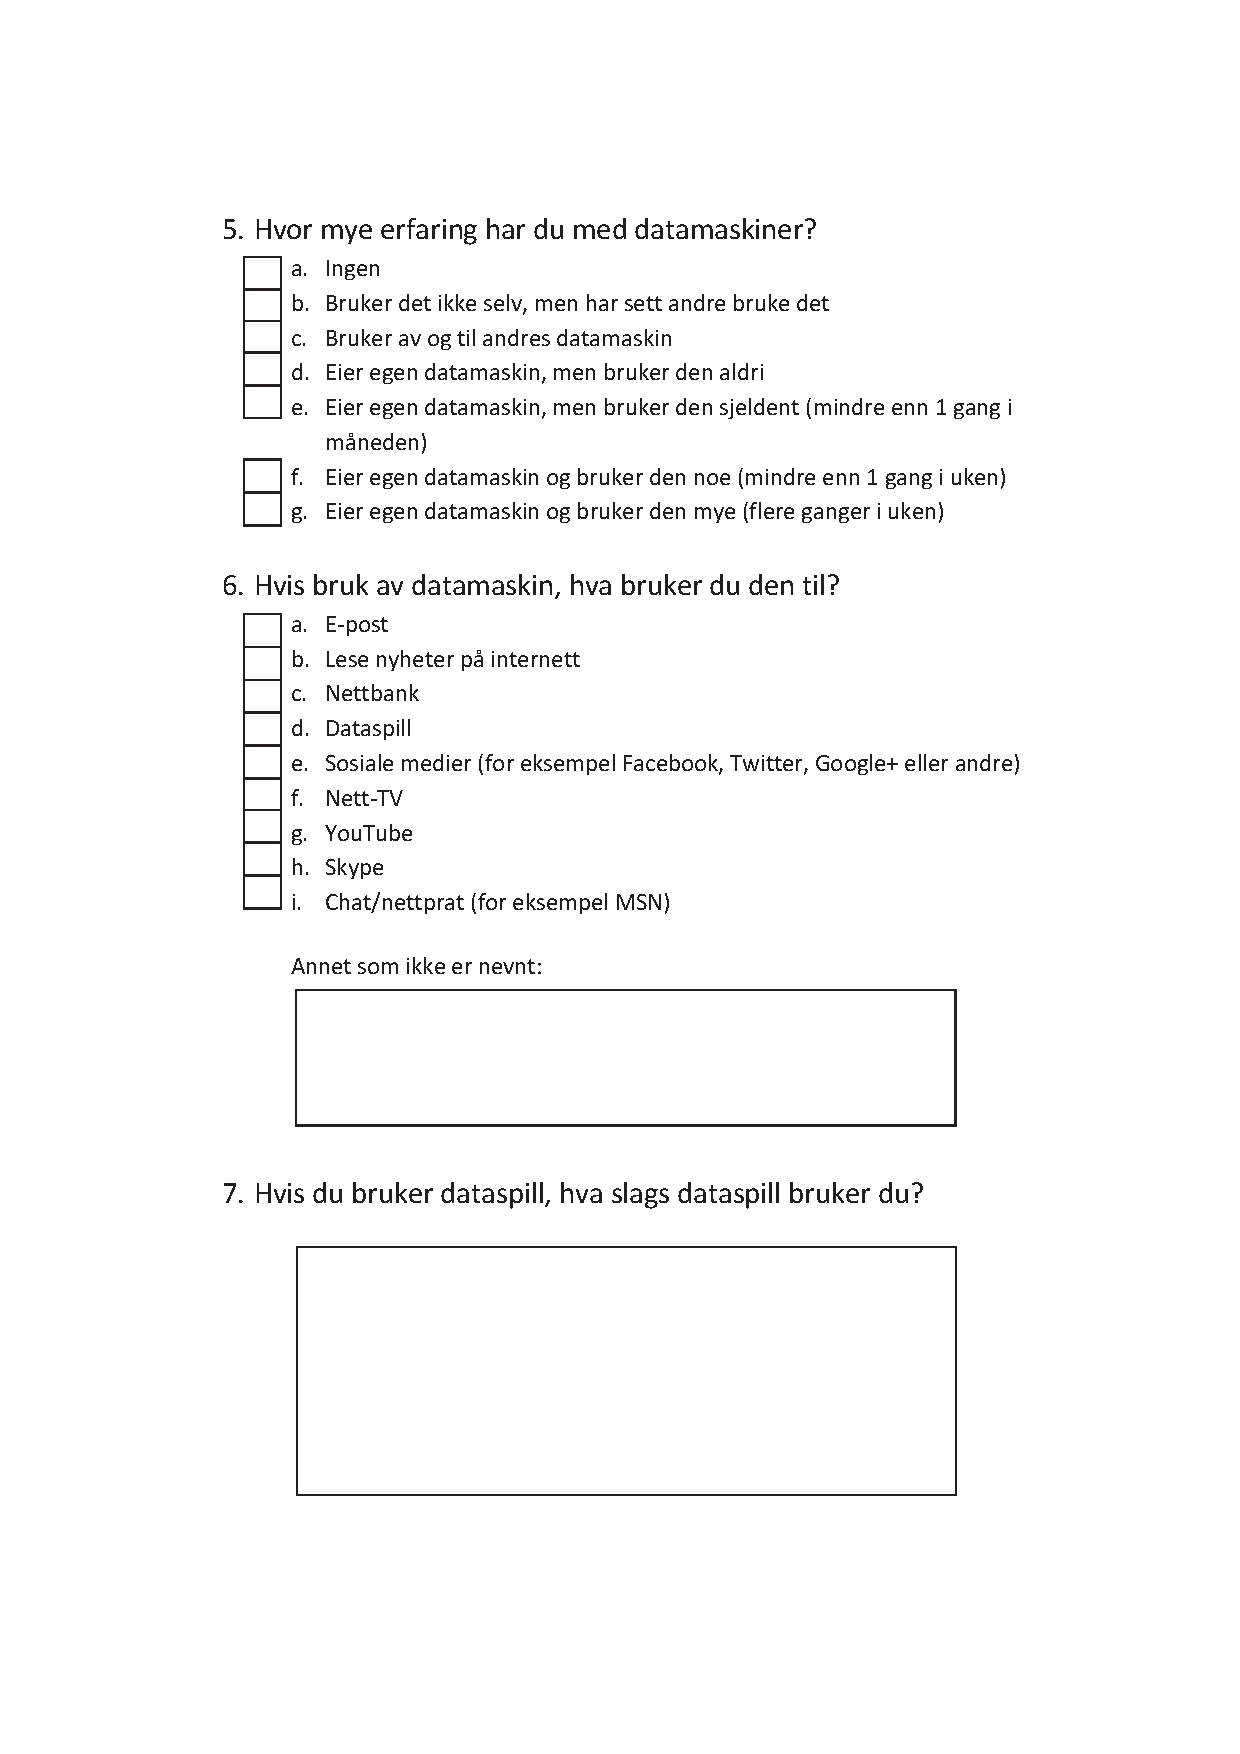
\includegraphics[scale=0.65]{SU2.pdf}}
\end{figure}  
\begin{figure}[H] 
\centering{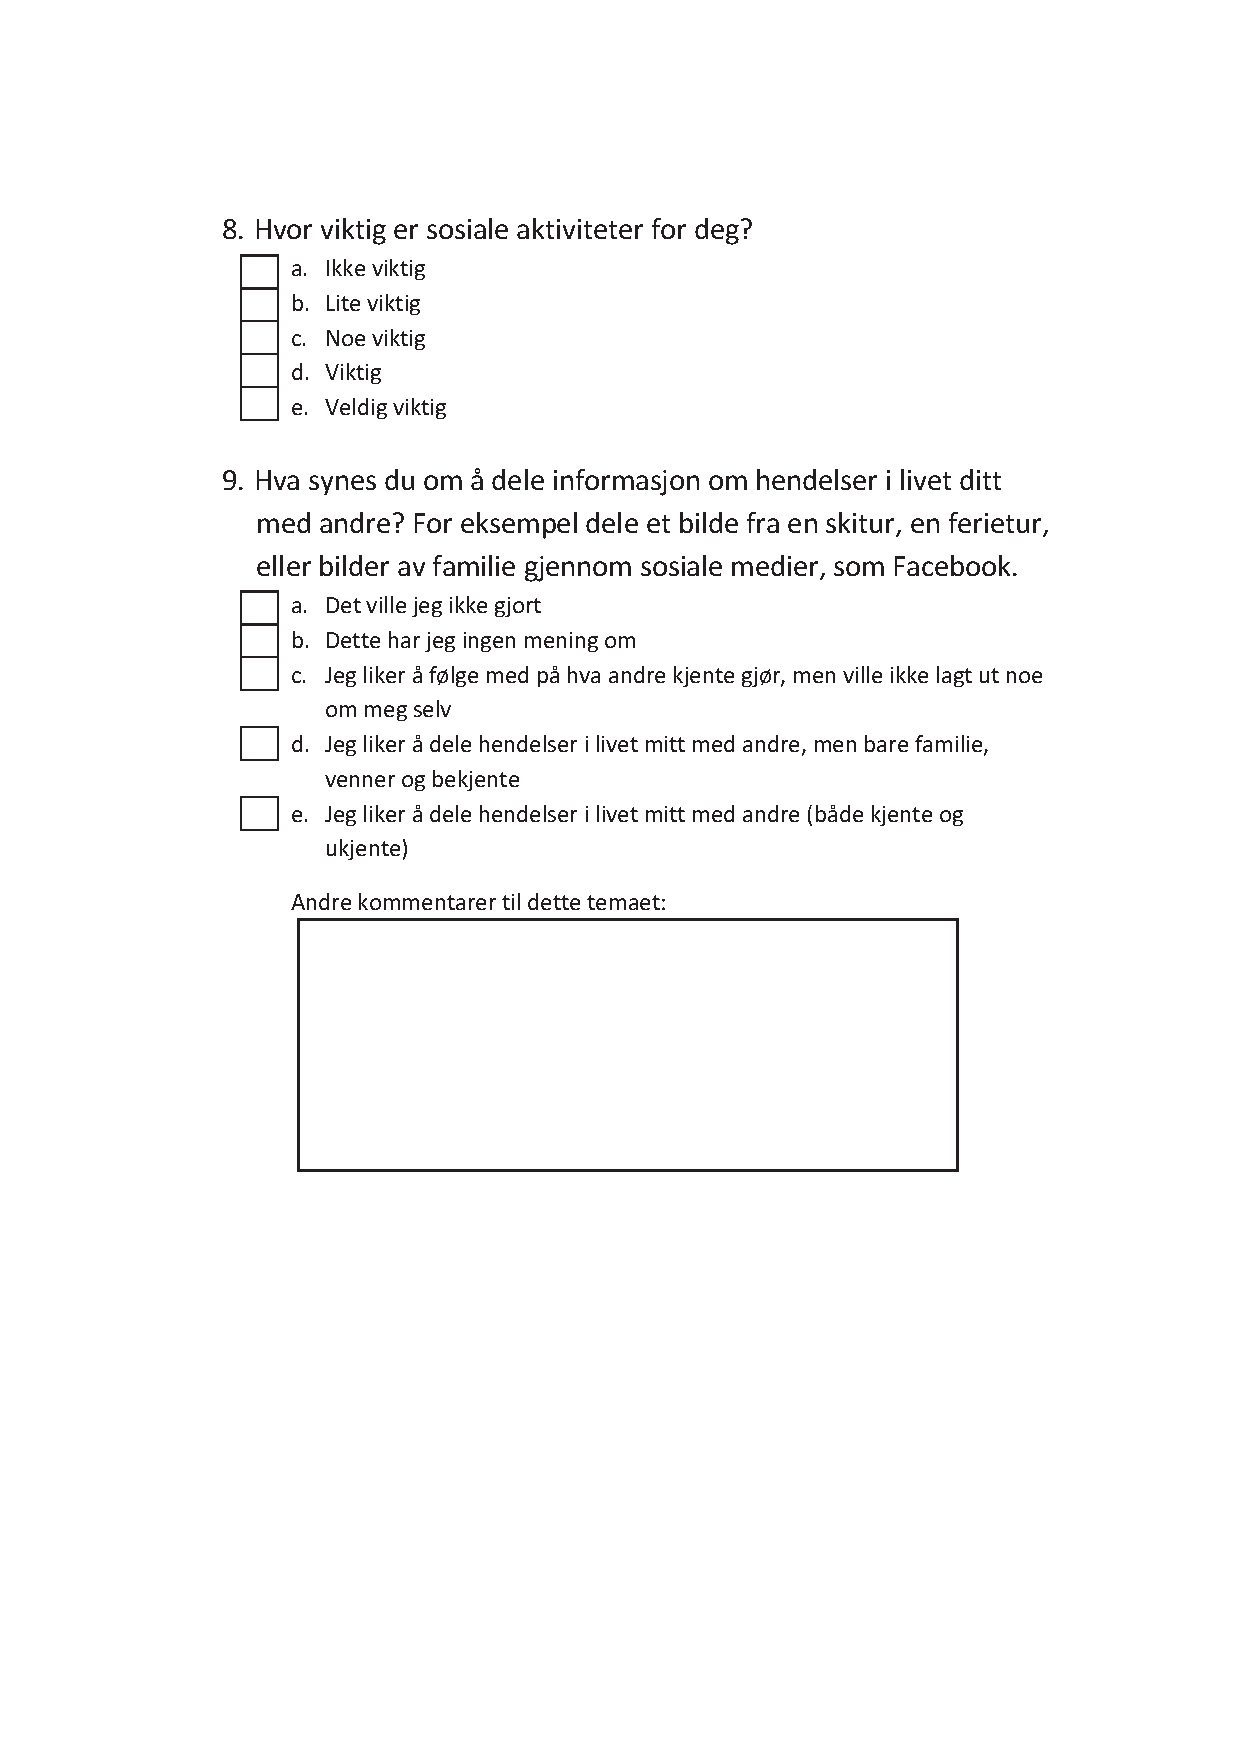
\includegraphics[scale=0.65]{SU3.pdf}}
\end{figure}  
\begin{figure}[H] 
\centering{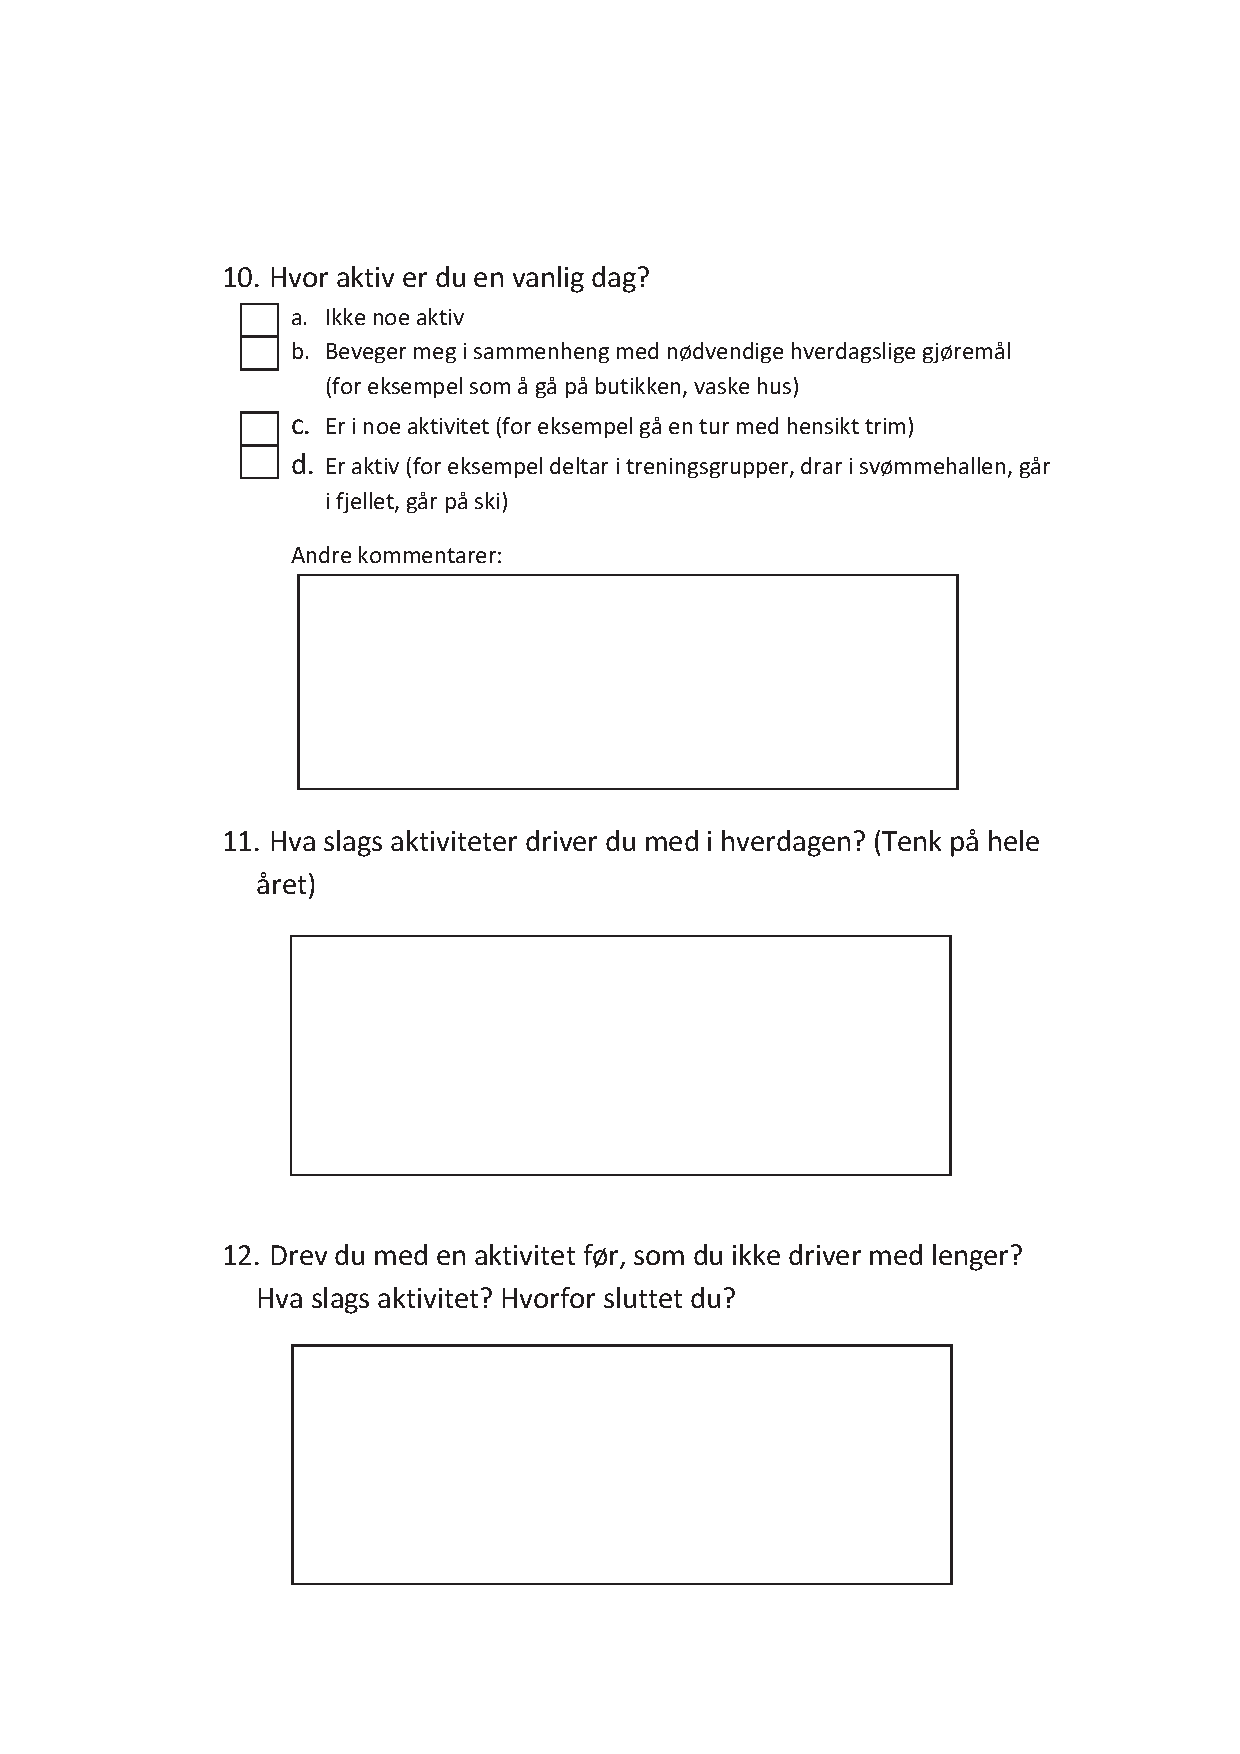
\includegraphics[scale=0.65]{SU4.pdf}}
\end{figure}  
\begin{figure}[H] 
\centering{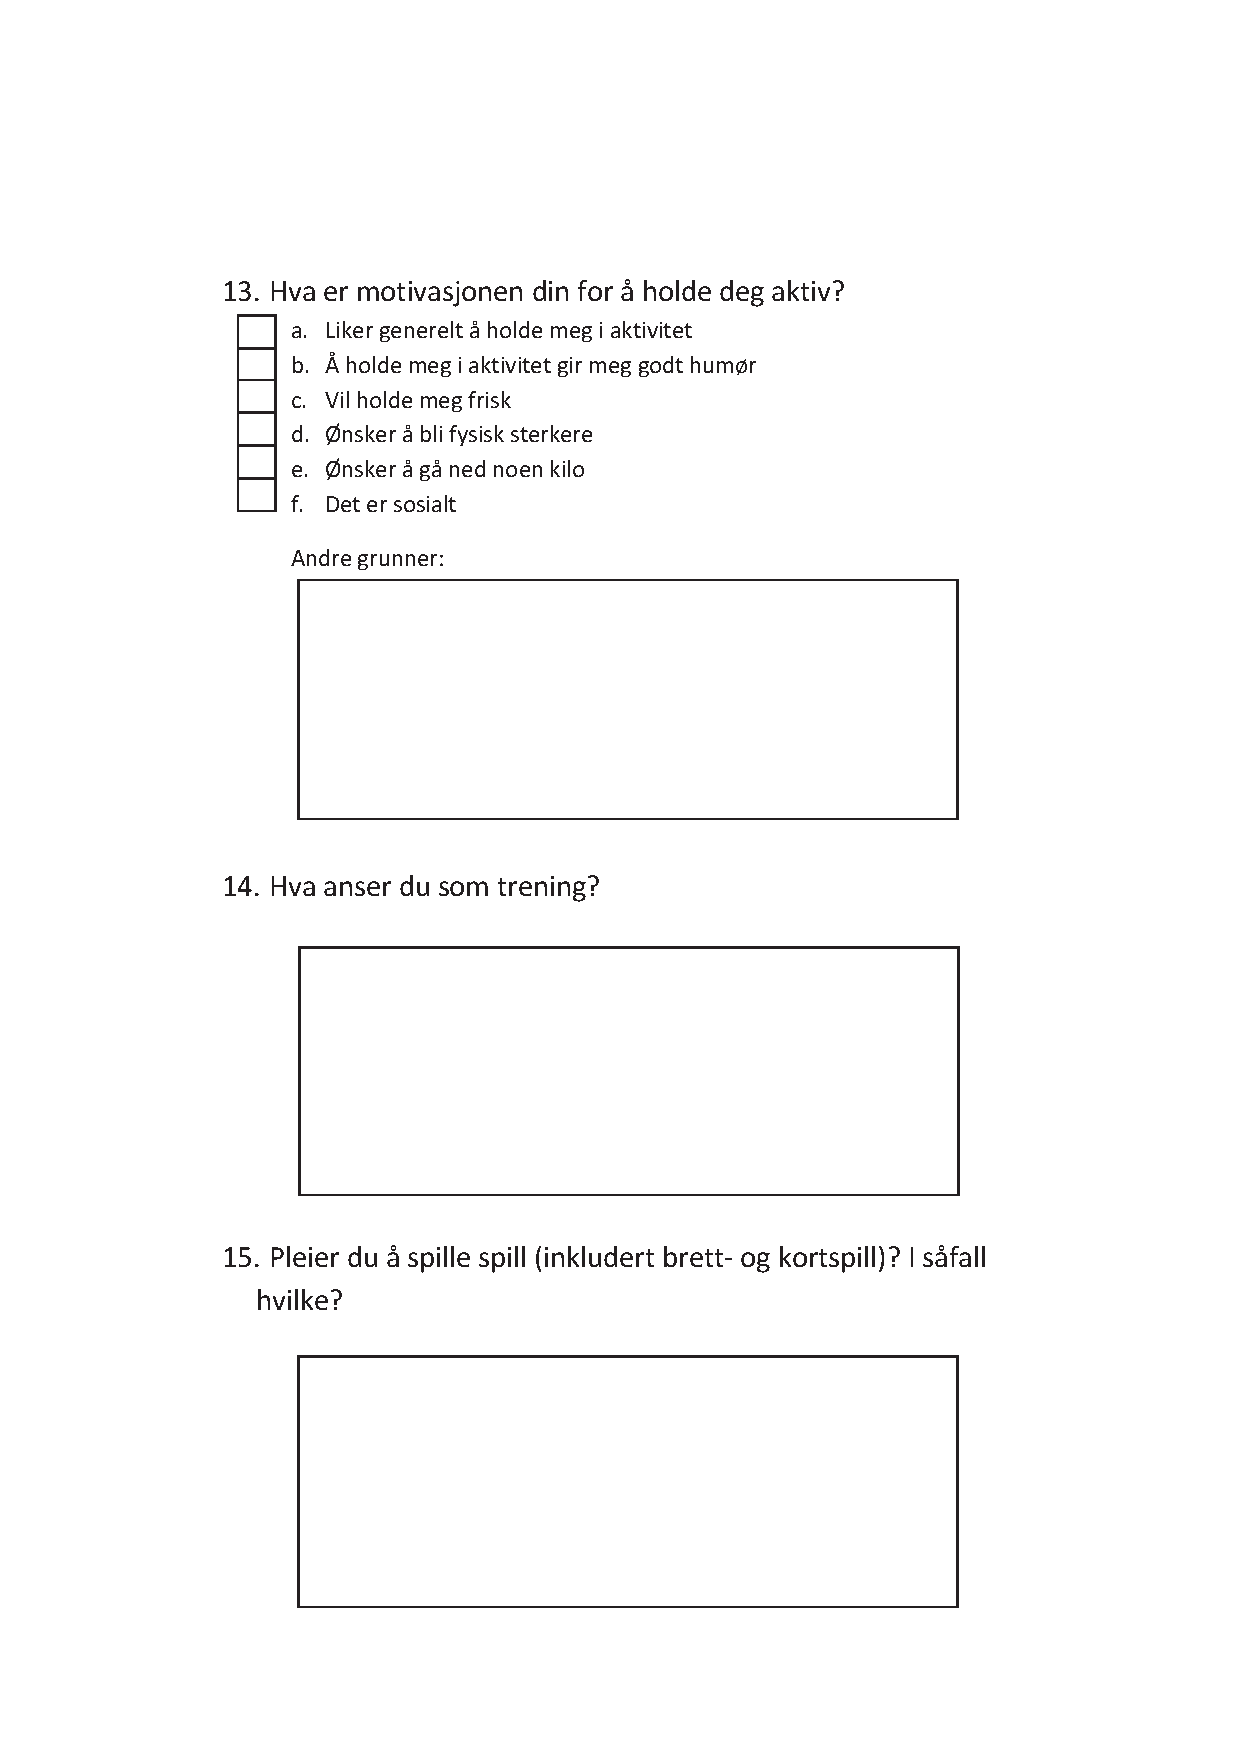
\includegraphics[scale=0.65]{SU5.pdf}}
\end{figure}  
\begin{figure}[H] 
\centering{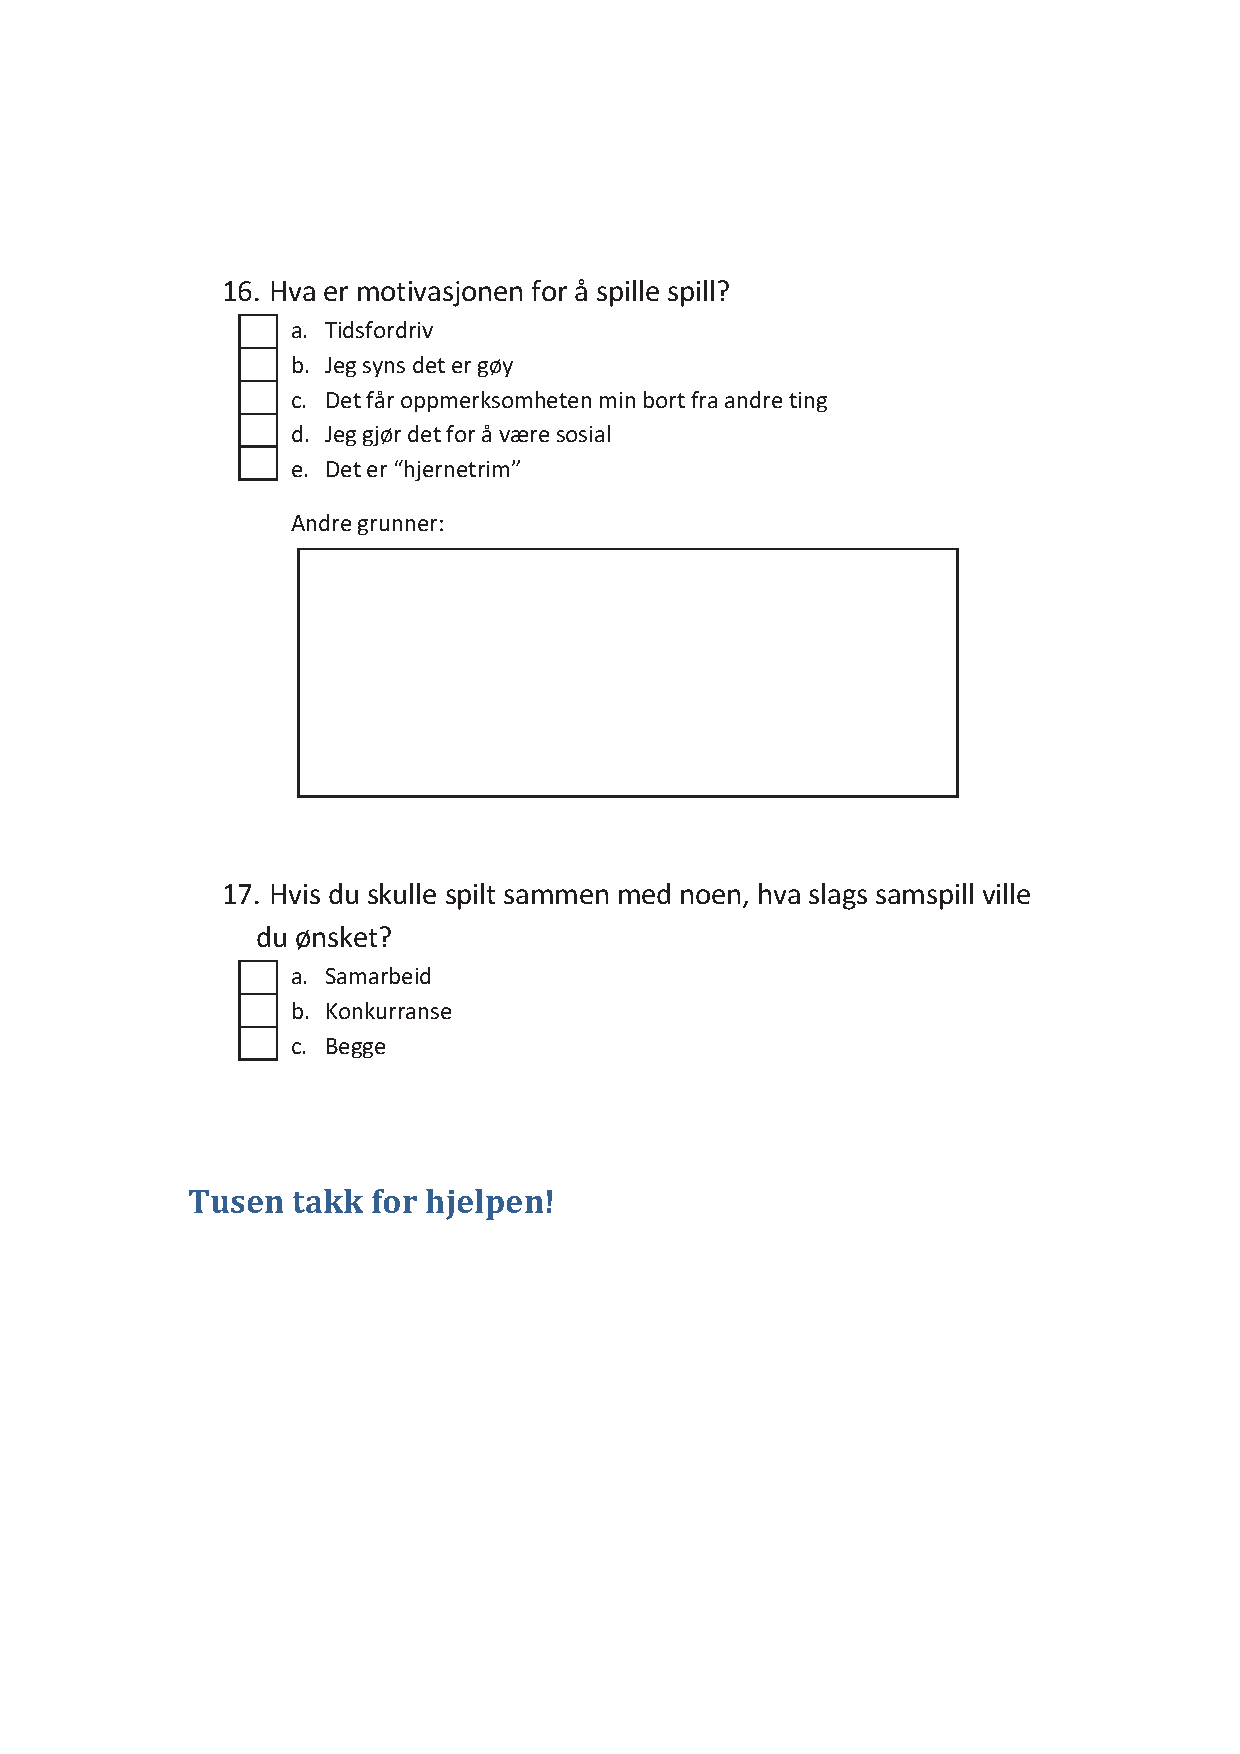
\includegraphics[scale=0.65]{SU6.pdf}}
\end{figure}  

\newpage
\section*{Appendix H - Interview Guide for the Focus Group Interview in Workshop 1}
\label{app:interviewGuide}
\begin{figure}[H] 
\centering{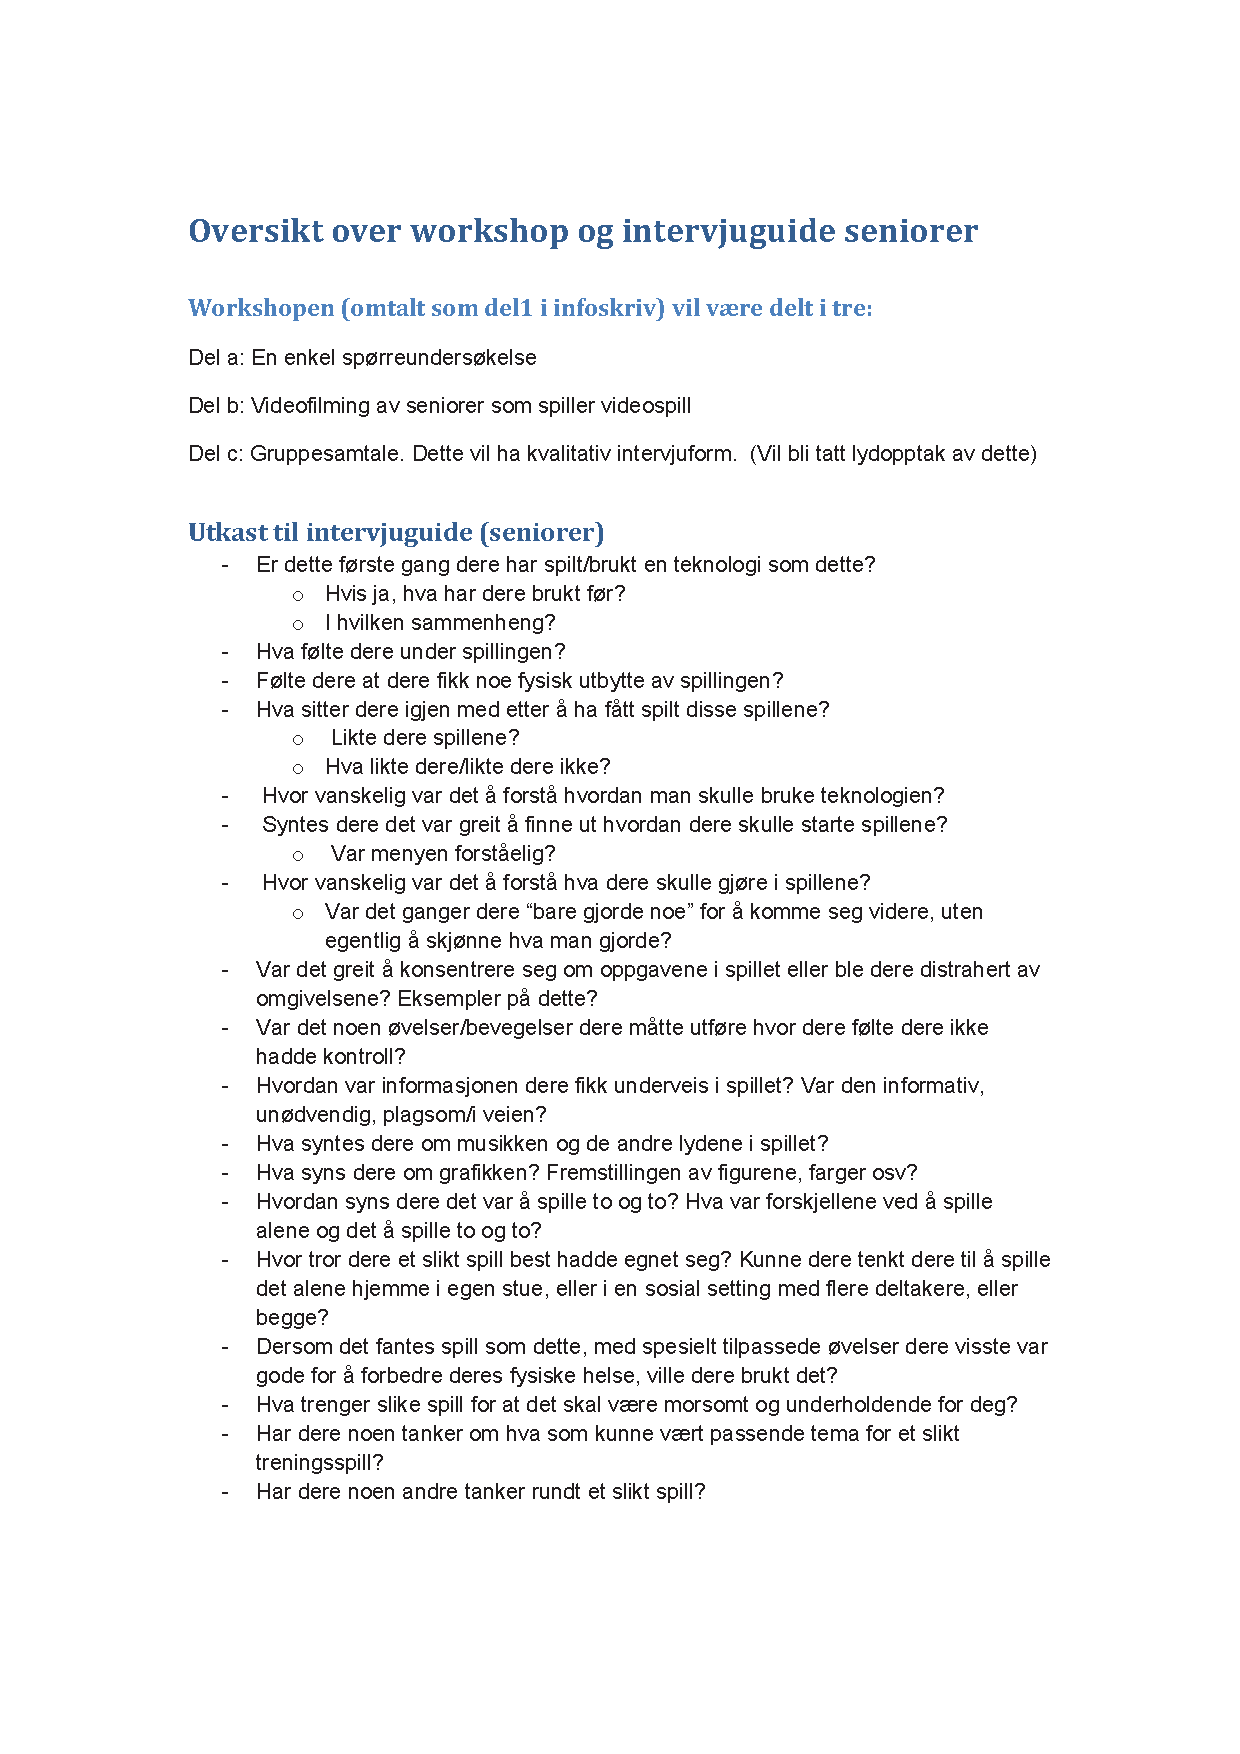
\includegraphics[scale=0.65]{questions.pdf}}
\end{figure}  

\newpage
\section*{Appendix I - Interview Guide for the Focus Group Interview in Workshop 2}
\label{app:interviewGuide2}
\begin{figure}[H] 
\centering{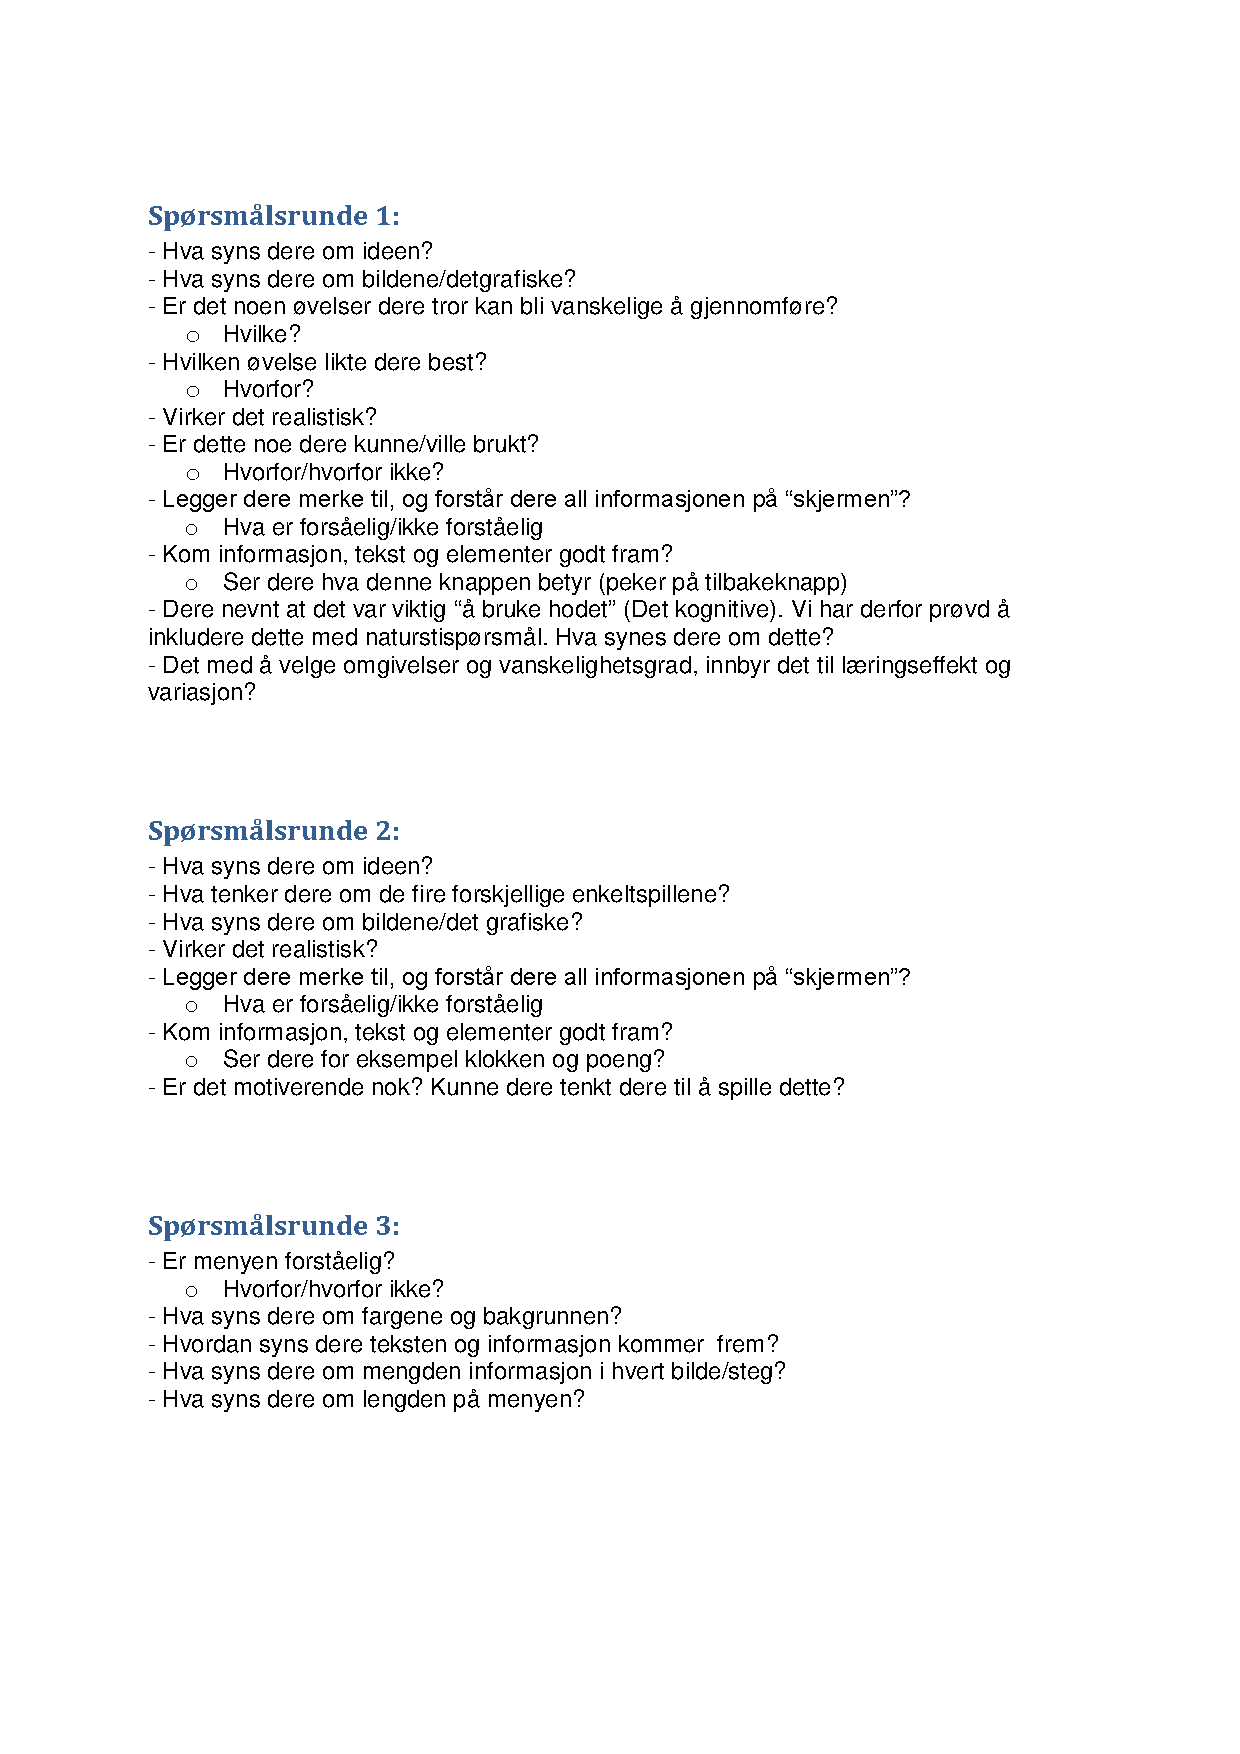
\includegraphics[scale=0.6]{interviewws2.pdf}}
\end{figure}

\newpage
\section*{Appendix J - Non-Functional Requirement not Included in the Exergame}

\begin{table} [H]
\label{tab:nfunc2}
\centering
\begin{tabular}{|l|l|}
\hline
3.1 & The system shall be able to run on both PC and Xbox. \\ \hline
3.2 & The system shall be easy to set up (physically).\\ \hline
3.3 & The system shall include Kinect functionality, like pausing \\ & a game by holding one arm out from the body. \\ \hline
3.4 & The system shall load within few seconds.\\ \hline
3.5 & The system shall be small in size and do not require too \\&  much space.\\ \hline
3.6 & The system shall not require too much capacity. It shall \\ & be able to run on a regular PC. \\ \hline
3.7 & The system shall not require too much power. \\ \hline
3.8 & The system shall avoid delay between the player's \\ & movement and action on the screen.\\ \hline
3.9 & The system shall ensure secure storage and sharing of \\ & profiles. \\ \hline
\end{tabular}
\caption[Miscellaneous non-functional requirements]{Miscellaneous non-functional requirements}
\end{table} 

\section{Quality of the Gathered Information}
\label{sec:discQuality}